\documentclass[a4paper,fleqn]{cas-dc}

\usepackage[utf8]{inputenc}
\usepackage[numbers,sort&compress]{natbib}
\usepackage{siunitx}
\usepackage{listings}
\usepackage{tikz}
\usepackage{enumitem}
\usetikzlibrary{arrows.meta,positioning,fit,shapes.geometric}
\graphicspath{{figures/}{els-cas-templates/}}
\setlength{\emergencystretch}{3em}
\hbadness=10000

% Revision round 3 markup (reviewer comments 4.1--4.3, broken ref, availability).
\providecommand{\revC}[1]{{\color{magenta}#1}}

% Revision round 4 markup (referee report M1--M12 and minor comments).
\providecommand{\revD}[1]{{\color{green!50!black}#1}}

\hypersetup{%
  colorlinks=true,
  linkcolor=black,
  citecolor=black,
  urlcolor=blue
}


\begin{document}
\let\WriteBookmarks\relax
\def\floatpagepagefraction{1}
\def\textpagefraction{.001}

\shorttitle{Reproducible Edge-to-Cloud Research Infrastructure}
\shortauthors{D'Agati et~al.}

\title[mode=title]{\texorpdfstring{A Reproducible Edge-to-Cloud Infrastructure\\ for Sustainable Orchestration of Embedded WebAssembly IoT Devices}{A Reproducible Edge-to-Cloud Infrastructure for Sustainable Orchestration of Embedded WebAssembly IoT Devices}}

\author[unime, cini]{Luca D'Agati}\cormark[1]
\ead{ldagati@unime.it}

\author[unime, cini]{Giuseppe Tricomi}
\author[unime]{Fabio Orazio Mirto}
\author[unime,cini]{Francesco Longo}
\author[unime,cini]{Giovanni Merlino}
\address[unime]{Department of Engineering, University of Messina, Messina, Italy}
\address[cini]{CINI\@: National Interuniversity Consortium for Informatics, Rome, Italy}
%\address[bio]{Department of Biomedical, Dental, and Morphological and Functional Imaging Sciences, University of Messina, Messina, Italy}

\cortext[1]{Corresponding author.}

\begin{highlights}
\item Kubernetes CRDs express intent for constrained non-node IoT devices.
\item A TLS/CBOR gateway bridges cloud orchestration and embedded WASM execution.
\item Reconciliation policies preserve evidence ownership across cloud, fog, and edge.
% Removed: \item A 100-trial campaign reports 100\% transactional success (Wilson LB 96.3\%) and 1286.0~ms mean end-to-end latency.
\item {\color{red}A 100-trial campaign reports 100\% transactional success (Wilson LB 96.3\%) and 1286.0~ms mean end-to-end latency for a minimal WASM module.}
% Removed: \item Measured southbound control traffic is 1728~B/h per device; gateway mediation averages under 5~MiB RAM\@.
\item {\color{red}Steady-state application-layer heartbeat traffic is 1728~B/h per device, excluding TLS and lower-layer overhead; gateway mediation averages under 5~MiB RAM\@.}
\end{highlights}
\begin{comment}

\begin{abstract}
Cloud\textendash{}Fog\textendash{}Edge infrastructures increasingly need to deploy and observe application logic across cloud services, gateways, and embedded Internet of Things (IoT) devices, but conventional cloud-native orchestration assumes Linux-class nodes with container runtimes, resident agents, and sufficiently rich networking. This assumption leaves a gap for constrained endpoints that must remain lightweight while still requiring secure attachment, life-cycle accountability, and reproducible evidence for sustainable research infrastructures. This work addresses the problem of expressing Kubernetes deployment intent for devices that cannot operate as Kubernetes nodes and translating that intent into verifiable embedded execution. We propose a Kubernetes-native framework that models devices, applications, and gateways through Custom Resource Definitions (CRDs) and uses a gateway-mediated control path to bind device identity, supervise liveness, dispatch WebAssembly (WASM) workloads, and report execution evidence back to the control plane. The gateway acts as the semantic boundary between declarative cloud state and constrained device protocols, preserving device simplicity while maintaining status ownership in Kubernetes. The framework is evaluated on a K3s-based test bed with emulated embedded targets and a complete enrollment-to-deployment workflow. % Removed: Across 100 independent trials, enrollment, heartbeat supervision, deployment, and transactional completion all succeeded (Wilson 95\% lower bound 96.3\%). Mean end-to-end latency is 1185.8~ms (95\% CI 1152.8--1218.7~ms). Measured southbound control traffic is 1728~B/h per device at a 25~s heartbeat period;
{\color{red}Across 100 repeated enrollment-to-deployment trials started from a known logical state, enrollment, heartbeat observability, deployment, and transactional completion all succeeded (Wilson 95\% lower bound 96.3\%). For the minimal 33~B WASM test module, mean end-to-end orchestration latency is 1286.0~ms (95\% CI 1226.4--1345.6~ms). Steady-state application-layer heartbeat traffic is 1728~B/h per device at a 25~s heartbeat period, excluding TLS and lower-layer overhead;} the gateway pod averages under 5~MiB RAM and 3~millicores CPU with one TLS-connected device, while {\color{red}the evaluated device firmware occupies 397~KiB of flash and approximately 264~KiB of static RAM, and the endpoint carries no kubelet or container runtime}. For sustainable digital research infrastructures, the framework therefore provides a reproducible, measurement-ready substrate for energy-aware placement, instrumentation, and green experimentation policies. % {\color{red}without claiming direct energy or carbon reduction in this evaluation}.
\end{abstract}
\end{comment}

\begin{abstract}
Cloud--Fog--Edge infrastructures increasingly need to deploy and observe application logic across cloud services, gateways, and embedded IoT devices, but conventional cloud-native orchestration assumes Linux-class nodes with container runtimes, resident agents, and rich networking. This leaves a gap for constrained endpoints that must remain lightweight while requiring secure attachment, life-cycle accountability, and reproducible evidence for sustainable research infrastructures. This work addresses the problem of expressing Kubernetes deployment intent for devices that cannot operate as Kubernetes nodes, and translating that intent into verifiable embedded execution. We propose a Kubernetes-native framework that models devices, applications, and gateways through Custom Resource Definitions (CRDs) and uses a gateway-mediated control path to bind device identity, supervise liveness, dispatch WebAssembly (WASM) workloads, and report execution evidence to the control plane. The gateway acts as the semantic boundary between declarative cloud state and constrained device protocols, preserving device simplicity while maintaining status ownership in Kubernetes. The framework is evaluated on a K3s-based test bed with emulated embedded targets across a complete enrollment-to-deployment workflow. Across 100 repeated trials, enrollment, heartbeat supervision, deployment, and transactional completion all succeeded. %(Wilson 95\% lower bound 96.3\%), with mean end-to-end latency of 1185.8~ms (95\% CI 1152.8--1218.7~ms). 
Heartbeat traffic stays under 2~KB/h per device, gateway pod footprint remains in the single-digit MiB and single-digit millicores, and the evaluated device firmware fits within 400~KiB of flash with no kubelet or container runtime. For sustainable research infrastructures, the framework provides a reproducible, measurement-ready substrate for energy-aware placement, instrumentation, and green experimentation policies.
\end{abstract}

\begin{keywords}
Cloud\textendash{}Fog\textendash{}Edge continuum \sep{} digital research infrastructures \sep{} sustainable orchestration \sep{} green experimentation \sep{} Internet of Things \sep{} WebAssembly \sep{} embedded systems \sep{} Kubernetes
\end{keywords}


\ExplSyntaxOn%
\bool_gset_true:N \g_stm_nologo_bool
\ExplSyntaxOff%
\begin{NoHyper}
\maketitle
\end{NoHyper}

\input{sections/02_introduction}
\section{Related Work}\label{sec:related-work}

This section reviews prior work along the axes that motivate the design in Sections~\ref{sec:problem}--\ref{sec:implementation}: edge orchestration, constrained execution, secure IoT communication, reconciliation semantics, and reproducible evaluation. The main gap across these areas is the lack of an end-to-end path from Kubernetes-style declarative intent to verifiable execution on constrained embedded devices that cannot act as ordinary cluster nodes.

\subsection{Cloud-Native Edge and IoT Orchestration}
Foundational work on fog and edge computing established the need to move computation, storage, and control closer to data sources in order to reduce latency, improve locality, and support cyber-physical applications~\cite{bonomi_fog,shi_edge,satyanarayanan_edge,chiang_fog}. Kubernetes has become the dominant orchestration substrate for cloud-native services because it provides declarative resource management, controllers, reconciliation loops, and extensibility through Custom Resource Definitions (CRDs) and operators~\cite{kubernetes,kubernetes_operators}. Lightweight distributions such as K3s and MicroK8s reduce deployment overhead and make cluster-style operation feasible at smaller sites~\cite{k3s,microk8s}.

Several systems extend Kubernetes semantics toward the edge. KubeEdge moves parts of Kubernetes control closer to edge nodes, OpenYurt targets cloud-edge application management, Akri discovers and exposes leaf devices to Kubernetes, and Krustlet explored WebAssembly workloads as Kubernetes-scheduled units~\cite{kubeedge,openyurt,akri,krustlet}. Recent Kubernetes-native IoT orchestration based on Stack4Things (S4T), CRDs, and Crossplane abstractions similarly demonstrates the value of declarative resource management for IoT deployments~\cite{dagati_iot_orchestration_s4t}. \revC{That line has since been extended toward a deviceless Function-as-a-Service model, in which users deploy and invoke functions according to capability, location, and load without managing the underlying devices, using Nuclio as the serverless runtime on edge workers and WebSocket tunnelling to reach nodes behind NATs or firewalls~\cite{mirto_deviceless_faas}. That design shares the goal of removing device-level management from the user, but its edge workers are Linux single-board hosts running a container-based function runtime, and the tunnelled node remains the unit of execution; the endpoint considered here executes a WASM module under Zephyr/WAMR with no operating-system userspace, container runtime, or cluster agent, so the mediation boundary sits at the gateway rather than at the device itself.} These approaches motivate the present work, but they generally assume Linux-class edge hosts, gateway nodes, container-compatible execution environments, device plugins, or platform services attached to capable nodes. The target considered here is narrower and more constrained: an embedded endpoint that cannot run a kubelet, container runtime, Kubernetes agent, or full cloud-native network stack.

IoT middleware and industrial edge platforms provide additional context. EdgeX Foundry, FIWARE, oneM2M, OMA Lightweight M2M, and OPC UA address aspects of device modeling, interoperability, telemetry, and industrial communication~\cite{edgex,fiware,onem2m,lwm2m,opcua}. These frameworks are broader than a single orchestration mechanism and often emphasize interoperability or application enablement rather than Kubernetes-native desired-state reconciliation. The contribution is therefore not another general IoT middleware layer, but a focused integration that links cloud-style intent, gateway-mediated secure control, and embedded WASM execution through explicit resource ownership.

\revD{The device twin, or shadow, pattern addresses the same problem from the platform side:
a cloud-resident document holds desired and reported state for a device that cannot be
queried directly, and a managed service reconciles the two as the device reconnects. AWS
IoT Greengrass~\cite{aws_greengrass}, Azure IoT Edge~\cite{azure_iot_edge} and the
LwM2M object model~\cite{lwm2m} have long provided this. The evidence model used here is
the same pattern; what differs is the location of the reconciliation point. In twin-based
platforms authoritative state lives in a proprietary service and reaches cluster tooling
through bridges. Here it is a Kubernetes resource from the outset, so status ownership,
admission control, watches and the controller pattern extend to constrained devices
directly, and a placement policy is an ordinary controller over the same objects.}

\subsection{Constrained Execution and Secure Communication}
Embedded and IoT operating systems provide the substrate on which constrained devices communicate and execute application logic. Zephyr, FreeRTOS, RIOT, and Contiki-NG represent different points in the design space for real-time behavior, connectivity, portability, and resource footprint~\cite{zephyr,freertos,riot,contiki}; TinyOS established the long-standing importance of event-driven and resource-aware design in sensor-network systems~\cite{tinyos}. These operating systems make embedded applications feasible, but they do not by themselves provide a cloud-side mechanism for expressing intent, binding identity, reconciling state, and verifying deployment outcomes.

WebAssembly adds a portable execution layer that can complement embedded operating systems. The original WebAssembly design emphasized safe, compact, and efficient portable code~\cite{haas_wasm,wasm_core}, while the WebAssembly System Interface (WASI) extended the ecosystem toward non-browser execution~\cite{wasi}. Runtime implementations such as WAMR, Wasmtime, WasmEdge, and wasm3 demonstrate that WASM can execute outside browsers and, in some cases, in resource-constrained settings~\cite{wamr,wasmtime,wasmedge,wasm3}. Container and cloud ecosystems have also begun to integrate WASM through projects such as runwasi and Spin~\cite{runwasi,spin}. These efforts establish runtime feasibility, but not operational orchestration: the unresolved question is how a cloud control plane can safely decide that a device should run a given module, transmit that intent through a trusted gateway, and receive evidence that execution and liveness match the requested state.

Secure IoT communication relies on standardized transport, object security, and compact serialization mechanisms. TLS 1.3 and DTLS 1.3 provide channel security~\cite{rfc8446,rfc9147}; CoAP and MQTT address lightweight application-layer communication~\cite{rfc7252,mqtt}; OSCORE and COSE provide object security and compact cryptographic containers~\cite{rfc8613,rfc9052}; and CBOR supports low-overhead binary serialization~\cite{rfc8949}. These mechanisms are complementary to the present work. A secure channel can protect messages in transit, but it does not determine which component owns reported state, when a device should be considered connected, or how a cloud resource should converge after a deployment acknowledgment.

\subsection{Reconciliation, Evaluation, and Positioning}
The operator pattern and Kubernetes controller model encode desired state, observe actual state, and repeatedly reconcile the two~\cite{kubernetes,kubernetes_operators}. In conventional clusters, this model works because nodes and workloads participate directly in the Kubernetes ecosystem. Edge systems complicate the model because connectivity can be intermittent, observations may be delayed, and devices may expose limited introspection. Prior platforms address parts of this challenge through edge agents, device twins, or local gateways~\cite{kubeedge,openyurt,akri,edgex,lwm2m}. For embedded targets, however, the gateway becomes more than a message forwarder: it is the semantic boundary between cloud resources and protocol-derived evidence.

Reproducible evaluation is equally important because physical hardware availability, network conditions, and manual setup can make embedded IoT experiments difficult to repeat. Large-scale experimental infrastructures such as SLICES highlight the role of programmable, shared scientific instruments for networking research~\cite{fdida2022slices}. Renode supports hardware-faithful emulation and multi-node embedded scenarios, while Cooja, ns-3, and OMNeT++ support repeatable simulation and network experimentation in wireless, sensor, and IoT research~\cite{renode,cooja,ns3,omnet}. The evaluation in this paper follows that direction by using an emulation-driven validation path and structured measurement records. This is appropriate because the main claim concerns end-to-end orchestration coherence rather than radio performance, energy consumption, or microarchitectural timing.

%Removed (ridondanza): Taken together, existing cloud-edge orchestration systems extend Kubernetes toward capable edge nodes; IoT middleware improves interoperability and telemetry; embedded operating systems and WASM runtimes make constrained execution feasible; and secure communication standards provide protected message exchange. The proposed framework connects these strands at a narrower integration point: a Kubernetes-native control plane expressing declarative deployment intent for an embedded-class endpoint that remains outside the cluster and reports execution evidence through a gateway.
Unlike middleware-centric approaches, the main abstraction is not a device model or telemetry bus, but the convergence between CRD intent, gateway evidence, and embedded WASM execution. The contribution is therefore best understood as a systems-integration study that combines explicit identity binding, gateway-mediated control, heartbeat-based liveness, CRD status convergence, and reproducible quantitative validation.

\begingroup
\color{red}
Table~\ref{tab:related-positioning} summarizes frameworks' characteristics. The comparison is qualitative because the surveyed systems target different layers of the edge continuum, but it clarifies the specific gap addressed here: preserving Kubernetes-native intent and reconciliation while keeping the embedded endpoint outside the cluster and still obtaining execution evidence.

\begin{table*}[pos=t]
\centering
\caption{Qualitative comparison relative to representative edge, IoT, and WASM orchestration approaches.}
\label{tab:related-positioning}
\footnotesize
\setlength{\tabcolsep}{3pt}
\begin{tabular}{p{0.17\linewidth} p{0.20\linewidth} p{0.20\linewidth} p{0.18\linewidth} p{0.17\linewidth}}
\toprule
\textbf{Approach} & \textbf{Primary abstraction} & \textbf{Assumed edge capability} & \textbf{Kubernetes integration} & \textbf{Gap for this work} \\
\midrule
KubeEdge/OpenYurt & Cloud-edge node and application management & Capable edge hosts or edge nodes with local agents & Extends Kubernetes control toward the edge & Too heavy for endpoints that cannot host cluster agents. \\
Akri/device-plugin style integration & Discovery and exposure of leaf devices & Kubernetes nodes near the device & Represents devices through cluster-attached resources & Does not make the constrained device itself a verifiable WASM execution target. \\
Krustlet/runwasi-style WASM execution & WASM workload as schedulable unit & Host able to participate in Kubernetes scheduling & Integrates WASM into Kubernetes workload execution & Targets worker-like execution environments rather than non-node embedded firmware. \\
\revC{Edge FaaS/deviceless serverless} & \revC{Function as deployment unit, with capability- and load-aware placement} & \revC{Linux single-board edge workers able to host a container-based function runtime} & \revC{Kubernetes- and Docker-based deployment of the function runtime} & \revC{Assumes an edge worker that can run a container runtime, not a non-node embedded endpoint.} \\
IoT middleware & Device model, telemetry, interoperability, and management & Gateway, server, or device-management infrastructure & May be bridged to cloud platforms but is not primarily a CRD reconciliation model & Provides broad IoT management, but not Kubernetes-native deployment intent to embedded WASM execution evidence. \\
This framework & CRD intent plus gateway-mediated evidence & Zephyr/WAMR endpoint with TLS/CBOR protocol support only & Uses CRDs, controllers, and status reconciliation without making the device a worker node & Focused on reproducible orchestration of constrained embedded WASM targets. \\
\bottomrule
\end{tabular}
\end{table*}
\endgroup

\section{Problem Formulation and Design Requirements}\label{sec:problem}

The platform addresses the following problem:
\begin{quote}
\emph{How can a Kubernetes-based control plane reliably express the intent that a constrained device should execute a specific WebAssembly module, route that intent through a secure gateway, and verify the resulting execution and liveness state, with measurable control-plane and southbound overhead compatible with sustainable research-infrastructure operation, without requiring the device to behave like a Kubernetes node?}
\end{quote}

Cloud orchestrators normally assume Linux-capable workers with container runtimes, cluster agents, and rich networking support. Embedded devices instead provide limited compute, memory, and network functionality, but they still need comparable guarantees for identity, observability, and life-cycle accountability. The framework therefore treats orchestration as an end-to-end translation problem between cloud intent, gateway-mediated protocol control, and edge-side WASM execution.

\subsection{Design Pillars}
The problem management is structured on three pillars, standing on the three level in which framework acts: 
\begin{itemize}
    \item At the resource-model level, Kubernetes assumes a declarative control plane with explicit status ownership, whereas embedded deployments often rely on imperative, device-local procedures that are opaque to the cloud.
    \item At the transport level, constrained devices need lightweight and secure communication paths, but the cloud side requires rich enough semantics to express enrollment, liveness, and application control.
    \item Operationally, even when protocol messages are correct, reconciliation logic must interpret transient conditions conservatively to avoid reporting an incorrect device state.
\end{itemize}
  

\subsection{Design Requirements}
These pillars lead to a compact set of requirements. Desired and observed state for devices, applications, and gateways must remain represented in Kubernetes resources. Enrollment must occur over a protected channel with auditable binding between transport-level identity and platform-level resource identity. The application life cycle must use a format usable across cloud, fog, and constrained edge targets, motivating WebAssembly as a common execution abstraction. Runtime evidence must confirm enrollment, heartbeat-based liveness, deployment status, and gateway association without manual inspection of device internals. For digital research infrastructures, the same evidence model should expose where workload placement, liveness, and execution outcomes can later be correlated with site-level power or carbon signals. Finally, the complete stack must deploy and test in a commodity research environment.

\begingroup
\color{red}
Table~\ref{tab:requirements-traceability} makes these requirements explicit and links each one to the architectural decision and evaluation observable used later in the paper. 
%This traceability is important because the system is not evaluated as a generic IoT middleware platform, but as an orchestration path whose correctness depends on agreement between cloud resources, gateway evidence, and device-side execution. A requirement is therefore considered satisfied only when the corresponding design element leaves an observable artifact in the control plane or in the measurement record.

\begin{table*}[pos=t]
\centering
\caption{Traceability between design requirements, architectural decisions, and evaluation observables.}
\label{tab:requirements-traceability}
\footnotesize
\setlength{\tabcolsep}{3pt}
\begin{tabular}{p{0.17\linewidth} p{0.30\linewidth} p{0.25\linewidth} p{0.20\linewidth}}
\toprule
\textbf{Requirement} & \textbf{Rationale} & \textbf{Design consequence} & \textbf{Evaluation observable} \\
\midrule
R1: Declarative intent & Operators need a durable statement of what should run even when a device is offline or temporarily unreachable. & Device, Application, and Gateway state is represented through Kubernetes CRDs rather than through ephemeral gateway memory alone. & Application desired state, Device phase, Gateway association, and status convergence. \\
R2: Identity binding & A protected channel is insufficient unless the endpoint is bound to the expected platform identity. & The gateway validates enrollment material before associating a TLS session with a Device resource. & Enrollment success, expected identity match, and gateway runtime view. \\
R3: Lightweight edge execution & Constrained endpoints cannot host kubelet, container runtimes, or Linux userspace services. & The device firmware executes portable WASM modules through WAMR on Zephyr. & Firmware footprint, WASM deployment result, and absence of edge cluster agents. \\
R4: Evidence-driven status & Control-plane state must describe observed execution rather than only command dispatch. & Gateway-propagated acknowledgments and results are treated as status evidence. & Deployment phase, execution outcome, heartbeat freshness, and transactional success count. \\
R5: Conservative liveness & Intermittent visibility must not immediately erase the latest valid attachment state. & Controllers avoid interpreting a single stale or incomplete observation as definitive disconnection. & Heartbeat observability, connectivity state, and cross-layer evidence checks. \\
R6: Reproducible sustainability baseline & Later energy and carbon policies require a repeatable orchestration substrate with known overhead. & The testbed records wire size, firmware footprint, and pod-level resource samples. & Bytes per hour per device, firmware flash/RAM footprint, gateway RAM, and gateway CPU. \\
\bottomrule
\end{tabular}
\end{table*}
\endgroup

%Secure attachment without unified state would remain difficult to operate; unified state without secure attachment would be insecure by construction; and either property without runtime evidence would leave operators unable to trust the control plane. 
Communication, orchestration, and status management are therefore co-designed rather than layered opportunistically. Embedded devices are not trusted to manage cluster state directly, and Kubernetes is not expected to maintain device sessions directly: a managed gateway acts as the trusted fog-layer mediation point while the control plane remains authoritative for desired state.

\input{sections/05_architecture}
\section{Protocol and Reconciliation}\label{sec:protocol}

\subsection{Southbound Life-Cycle}
The southbound protocol uses framed CBOR messages over TLS\@. It is compact enough for embedded-class clients, but still supports identity binding, acknowledgments, liveness evidence, and application deployment. The life-cycle has three phases: enrollment, heartbeat-based supervision, and resource-driven WASM deployment.

Enrollment establishes the transition from a protected transport session to a platform-recognized device identity:
\begin{enumerate}
    \item The device opens a protected session with the gateway and requests enrollment.
    \item The gateway validates the request before proceeding.
    \item The device provides identity material that can be bound to a known platform resource, and signs a single-use gateway nonce to demonstrate that it holds the matching private key.
    \item The gateway verifies the signature and compares the material with the identity registered in the control plane.
    \item The device confirms that enrollment information has been received and that it is ready for managed operation.
    \item The gateway stores the device\textendash{}session association and updates the corresponding resource status.
\end{enumerate}

After enrollment, periodic heartbeats maintain liveness visibility. At the communication layer, they show that the protected channel and device remain responsive. At the control-plane layer, they provide evidence used to refresh reported connectivity and device phase. Missing or delayed observations are interpreted conservatively, so transient gaps do not immediately become disconnection events.

%Removed (ridondanza con Fig.~4): WASM deployment follows the same evidence-driven pattern, but starts from declarative intent rather than from device attachment: \begin{enumerate} \item An operator or higher-level service declares that a target device should run a specific WASM workload. \item The control plane observes the desired state and identifies the mediation path through the appropriate gateway. \item The gateway translates the deployment intent into compact protected messages for the device. \item The device firmware uses its embedded WASM runtime to load and start the workload. \item The device returns execution evidence or an error indication to the gateway. \item The gateway propagates the reported outcome back into the control-plane status visible to operators. \end{enumerate}
\revD{WASM deployment follows the same evidence-driven pattern but starts from declarative
intent: an operator declares that a target device should run a workload, the control plane
resolves the mediation path, the gateway translates the intent into protected messages, the
device loads the module through its embedded runtime and returns execution evidence, and the
gateway propagates the outcome into control-plane status (Figure~\ref{fig:deployment-workflow}).}

\begin{figure}
\centering
\resizebox{0.82\columnwidth}{!}{%
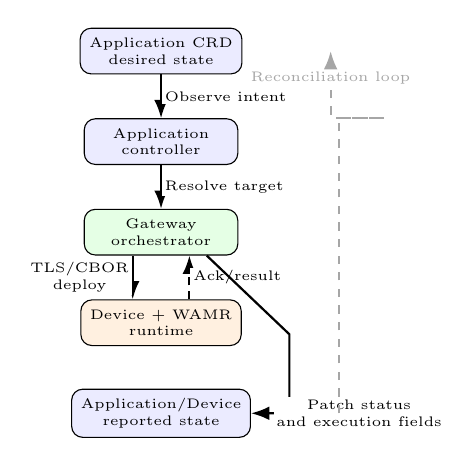
\begin{tikzpicture}[
    box/.style={draw,rounded corners,align=center,minimum width=1.95cm,minimum height=0.58cm,font=\tiny},
    flow/.style={-Latex,thick},
    returnflow/.style={-Latex,thick,densely dashed},
    feedback/.style={-Latex,thick,dashed,gray!70},
    note/.style={font=\tiny,align=center,fill=white,inner sep=1pt}
]
\node[box,fill=blue!8] (intent) at (0,0) {Application CRD\\desired state};
\node[box,fill=blue!8] (controller) at (0,-1.15) {Application\\controller};
\node[box,fill=green!10] (gateway) at (0,-2.3) {Gateway\\orchestrator};
\node[box,fill=orange!12] (device) at (0,-3.45) {Device + WAMR\\runtime};
\node[box,fill=blue!8] (status) at (0,-4.6) {Application/Device\\reported state};

\draw[flow] (intent) -- node[right,note]{Observe intent} (controller);
\draw[flow] (controller) -- node[right,note]{Resolve target} (gateway);
\draw[flow] ([xshift=-0.36cm]gateway.south) -- node[left,note]{TLS/CBOR\\deploy} ([xshift=-0.36cm]device.north);
\draw[returnflow] ([xshift=0.36cm]device.north) -- node[right,note]{Ack/result} ([xshift=0.36cm]gateway.south);
\draw[flow] ([xshift=0.58cm]gateway.south) -- ++(1.05,-1.0) |- node[pos=0.72,right,note]{Patch status\\and execution fields} (status.east);
\draw[feedback] ([xshift=1.12cm]status.east) |- ++(0.58,3.75) -| node[pos=0.72,above,note]{Reconciliation loop} ([xshift=1.12cm]intent.east);
\end{tikzpicture}%
}
\caption{Application deployment workflow and status-reconciliation loop.}%
\label{fig:deployment-workflow}
\end{figure}

Figure~\ref{fig:deployment-workflow} summarizes the deployment loop: the controller resolves intent, the gateway mediates the southbound command, the device reports an outcome, and the control plane reconciles status. This preserves the declarative pattern and remains compatible with retry, staged rollout, and multi-gateway scheduling policies.

\subsection{Protocol Sequences}
Figures~\ref{fig:enrollment-sequence} and~\ref{fig:deployment-sequence} summarize the southbound protocol interactions evaluated in Section~\ref{sec:evaluation}. The diagrams emphasize role ownership: the device initiates attachment and emits runtime evidence, the gateway validates and translates protocol events, and the Kubernetes control plane stores desired and reported state.

\begin{figure}
\centering
\resizebox{\columnwidth}{!}{%
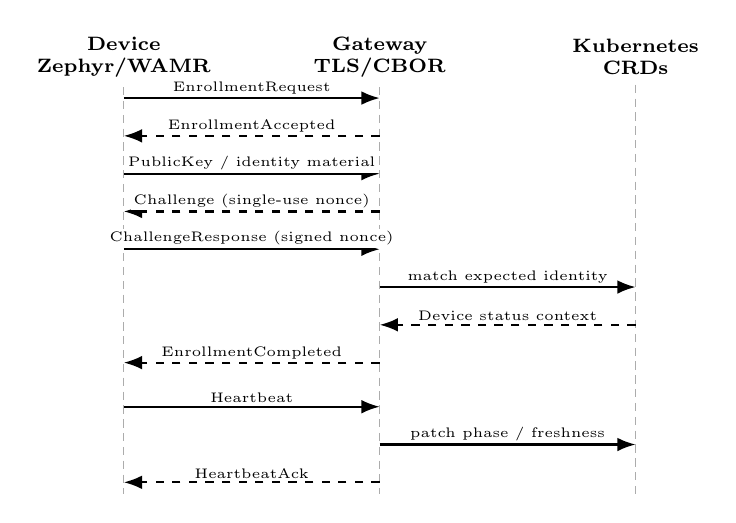
\begin{tikzpicture}[
    actor/.style={font=\scriptsize\bfseries,align=center},
    lifeline/.style={densely dashed,gray!65},
    msg/.style={-Latex,thick},
    ret/.style={-Latex,thick,dashed},
    note/.style={font=\tiny,align=center,fill=white,inner sep=1pt}
]
\node[actor] (device) at (0,0) {Device\\Zephyr/WAMR};
\node[actor] (gateway) at (3.25,0) {Gateway\\TLS/CBOR};
\node[actor] (control) at (6.5,0) {Kubernetes\\CRDs};

\draw[lifeline] (device) -- (0,-5.55);
\draw[lifeline] (gateway) -- (3.25,-5.55);
\draw[lifeline] (control) -- (6.5,-5.55);

\draw[msg] (0,-0.52) -- node[above,note]{EnrollmentRequest} (3.25,-0.52);
\draw[ret] (3.25,-1.00) -- node[above,note]{EnrollmentAccepted} (0,-1.00);
\draw[msg] (0,-1.48) -- node[above,note]{PublicKey / identity material} (3.25,-1.48);
\draw[ret] (3.25,-1.96) -- node[above,note]{Challenge (single-use nonce)} (0,-1.96);
\draw[msg] (0,-2.44) -- node[above,note]{ChallengeResponse (signed nonce)} (3.25,-2.44);
\draw[msg] (3.25,-2.92) -- node[above,note]{match expected identity} (6.5,-2.92);
\draw[ret] (6.5,-3.40) -- node[above,note]{Device status context} (3.25,-3.40);
\draw[ret] (3.25,-3.88) -- node[above,note]{EnrollmentCompleted} (0,-3.88);
\draw[msg] (0,-4.44) -- node[above,note]{Heartbeat} (3.25,-4.44);
\draw[msg] (3.25,-4.92) -- node[above,note]{patch phase / freshness} (6.5,-4.92);
\draw[ret] (3.25,-5.40) -- node[above,note]{HeartbeatAck} (0,-5.40);
\end{tikzpicture}%
}
\caption{Enrollment and heartbeat sequence. The device proves key possession by signing a single-use nonce before its evidence is reflected into Kubernetes status.}%
\label{fig:enrollment-sequence}
\end{figure}

\begin{figure}
\centering
\resizebox{\columnwidth}{!}{%
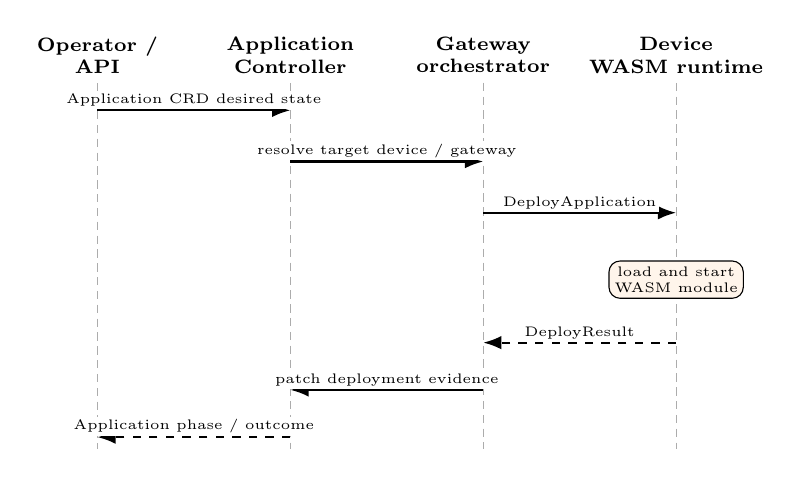
\begin{tikzpicture}[
    actor/.style={font=\scriptsize\bfseries,align=center},
    lifeline/.style={densely dashed,gray!65},
    msg/.style={-Latex,thick},
    ret/.style={-Latex,thick,dashed},
    note/.style={font=\tiny,align=center,fill=white,inner sep=1pt}
]
\node[actor] (operator) at (0,0) {Operator /\\API};
\node[actor] (control) at (2.45,0) {Application\\Controller};
\node[actor] (gateway) at (4.9,0) {Gateway\\orchestrator};
\node[actor] (device) at (7.35,0) {Device\\WASM runtime};

\draw[lifeline] (operator) -- (0,-5.0);
\draw[lifeline] (control) -- (2.45,-5.0);
\draw[lifeline] (gateway) -- (4.9,-5.0);
\draw[lifeline] (device) -- (7.35,-5.0);

\draw[msg] (0,-0.7) -- node[above,note]{Application CRD desired state} (2.45,-0.7);
\draw[msg] (2.45,-1.35) -- node[above,note]{resolve target device / gateway} (4.9,-1.35);
\draw[msg] (4.9,-2.0) -- node[above,note]{DeployApplication} (7.35,-2.0);
\node[draw,rounded corners,fill=orange!8,font=\tiny,align=center,inner sep=2pt] at (7.35,-2.85) {load and start\\WASM module};
\draw[ret] (7.35,-3.65) -- node[above,note]{DeployResult} (4.9,-3.65);
\draw[msg] (4.9,-4.25) -- node[above,note]{patch deployment evidence} (2.45,-4.25);
\draw[ret] (2.45,-4.85) -- node[above,note]{Application phase / outcome} (0,-4.85);
\end{tikzpicture}%
}
\caption{WASM deployment sequence. Declarative application intent is translated by the gateway into device execution and reconciled as application status.}%
\label{fig:deployment-sequence}
\end{figure}

%Removed (ridondanza): During enrollment, the decisive event is not the opening of a protected transport session alone, but the successful association between the device-provided identity material and the \texttt{Device} resource expected by the control plane. Heartbeats then refresh the same association by producing liveness evidence that the gateway can interpret before patching Kubernetes status. Deployment follows the complementary direction: the \texttt{Application} resource records desired state, the controller resolves the mediation path, and the gateway converts intent into a southbound command. The returned \texttt{DeployResult} is treated as execution evidence, not merely as a transport acknowledgment, only after this evidence is propagated does application status converge to the reported outcome.
\revD{The decisive event in enrollment is not the opening of a protected session but the
association between the device-provided identity material and the expected \texttt{Device}
resource, admitted only once possession of the matching private key is proved; heartbeats
then refresh that association. Deployment runs the complementary direction, and the
returned \texttt{DeployResult} is treated as execution evidence rather than as a transport
acknowledgment: application status converges only once that evidence is propagated.}

\subsection{Reconciliation Policy}
Protocol correctness becomes platform correctness only when message outcomes are interpreted consistently by the control plane. The framework therefore gives the gateway authority over protocol-derived observations and constrains controllers to reconcile those observations without overreacting to transient visibility gaps.

Integration testing exercised short-lived differences between gateway observations and control-plane status, confirming that liveness should not be inferred from a single incomplete observation. The resulting policy preserves the latest valid gateway association, avoids immediate disconnection when heartbeat evidence and transport visibility briefly diverge, and waits for a subsequent reconciliation cycle before treating the condition as a real state transition. Reconciliation policy is therefore part of the architecture rather than an incidental implementation detail.

\revD{Four constants govern the policy. The firmware emits a heartbeat every 25~s; the gateway
treats an association as stale after 90~s without one, evaluated on a 30~s sweep; Device
and Application controllers requeue every 30~s. The staleness threshold is $3.6\times$ the
emission period, so at least three consecutive heartbeats must be lost before a device
leaves \texttt{Connected} for \texttt{Unreachable}, detected with $\pm30$~s granularity.
Oscillation is precluded by construction rather than by damping: the timeout transition is
one-directional and only a fresh heartbeat restores \texttt{Connected}, so a single delayed
observation cannot produce a disconnect--reconnect cycle.}

\begingroup
\color{red}
\begin{table*}[pos=t]
\centering
%Removed (minore): \caption{Additive implementation-facing conventions for the validated gateway-mediated control path.}
\caption{\revD{Implementation-facing conventions for the validated gateway-mediated control path.}}
\footnotesize
\setlength{\tabcolsep}{3pt}
\begin{tabular}{p{0.18\linewidth} p{0.36\linewidth} p{0.36\linewidth}}
\toprule
\textbf{Element} & \textbf{Minimum evidence carried or recorded} & \textbf{Status/reconciliation use} \\
\midrule
Enrollment & Device identifier, firmware/runtime descriptor, device public-key material or fingerprint, gateway identifier, and freshness context for the protected session & The gateway binds the transport session to the expected \texttt{Device} resource before reporting connectivity or phase updates. \\
Heartbeat & Device identifier, gateway/session association, receive timestamp, and heartbeat freshness window & Controllers interpret heartbeat evidence conservatively: stale or missing observations do not overwrite the latest valid association until a subsequent reconciliation cycle confirms a state transition. \\
Deployment & Application identifier, target device, WASM artifact reference or payload hash, desired execution state, result status, and error or exit evidence when available & \texttt{Application} status converges only after gateway-propagated execution evidence; desired state remains intact when deployment evidence is missing, stale, or inconsistent. \\
Measurement record & Trial identifier, enrollment result, heartbeat-freshness check, deployment result, gateway runtime view, \texttt{Device} status, \texttt{Application} status, timeout outcome, and latency timestamps & A trial is counted as transactionally successful only when all evidence views agree; otherwise the trial is recorded as failed rather than inferred from a single eventually consistent field. \\
\bottomrule
\end{tabular}
\end{table*}
\endgroup

For reproducibility, the protocol messages evaluated here should therefore be read as typed CBOR records with explicit identity, freshness, target, artifact, and outcome fields, even when the diagrams show only message names. The implementation-facing invariant is that a transport acknowledgment alone is insufficient for success: Kubernetes status is updated only after the gateway has matched the device identity, preserved the gateway association, and propagated fresh deployment or liveness evidence.
%Removed (ridondanza): {\color{red}In the evaluated configuration, heartbeat freshness is interpreted relative to the configured 25~s firmware heartbeat period: a newly observed heartbeat refreshes the gateway association, while stale or missing observations are treated conservatively and do not immediately erase the last valid association until reconciliation confirms the transition. The protocol specification is intentionally minimal in this manuscript; a replication package should expose the concrete CRD schemas, CBOR field names, status enum values, timeout constants, and error codes used by the implementation.}


\section{Implementation}\label{sec:implementation}

The implementation combines Rust control-plane services with Zephyr-based device firmware and WAMR execution. The API server, gateway, and controllers are implemented in Rust, using its memory-safety guarantees and asynchronous networking support. Resource interaction follows Kubernetes controller and status-patching practices~\cite{kubernetes,kubernetes_operators}, allowing embedded endpoints to be managed as first-class resources without treating them as cluster nodes. On the device side, Zephyr provides the embedded networking and TLS substrate~\cite{zephyr}, while WAMR provides lightweight WASM execution on constrained targets~\cite{wamr}.

The reference deployment runs on K3s~\cite{k3s}. {\color{red}In the presented framework, K3s denotes the concrete lightweight Kubernetes distribution used for the experiments, whereas K8s/Kubernetes denotes the generic API, manifests, CRDs, and controller model implemented by the framework and reflected in the repository naming.} It uses namespace-scoped resources and locally built images, preserving real Kubernetes API and reconciliation semantics while remaining accessible on a single-node Linux environment for development, experimentation, and repeatable evaluation. The deployment includes the API services, dashboard, gateway/controller components, CRDs, and supporting services needed to exercise enrollment, deployment, and status propagation.

Responsibilities are distributed across specialized controllers rather than concentrated in a single service. Device-oriented reconciliation manages attachment state and gateway resolution. Application-oriented reconciliation interprets deployment intent and maps it to gateway actions. Gateway-oriented reconciliation maintains metadata needed for path resolution and status interpretation. This decomposition follows the CRD model and reduces the risk that unrelated concerns become coupled inside one control loop.

\begingroup
\color{red}
\subsection{Control-Plane Components}
The control-plane implementation is organized around a narrow API layer and a set of reconciliation workers. The API server is responsible for user-facing operations, validation of high-level requests, and creation or update of Kubernetes resources. It does not maintain authoritative device-session state. That responsibility is delegated to the gateway and reflected through CRD status fields, so that the Kubernetes API remains the persistent source of desired state and the gateway remains the source of southbound observations. This split prevents the dashboard or API server from becoming a hidden second control plane.

The Device controller watches Device resources and interprets gateway-reported attachment evidence. Its primary task is not to open device connections directly, but to maintain a consistent platform view: the selected gateway, the latest known connectivity phase, heartbeat freshness, and the last valid association between device identity and gateway session. The Application controller watches Application resources and turns a desired deployment into a gateway action only when the target device and mediation path can be resolved. The Gateway controller maintains gateway metadata and makes the mapping between cloud-side resources and fog-layer endpoints explicit. Table~\ref{tab:implementation-components} summarizes these responsibilities.

\begin{table*}[pos=t]
\centering
\caption{Implementation responsibilities across the validated stack.}
\label{tab:implementation-components}
\footnotesize
\setlength{\tabcolsep}{3pt}
\begin{tabular}{p{0.18\linewidth} p{0.32\linewidth} p{0.25\linewidth} p{0.17\linewidth}}
\toprule
\textbf{Component} & \textbf{Main responsibility} & \textbf{State written or observed} & \textbf{Failure containment} \\
\midrule
Dashboard and API server & Accept operator requests, validate high-level parameters, and create or update CRD objects. & Application desired state, Device metadata, and Gateway references. & No direct southbound session ownership. \\
Device controller & Interpret attachment, phase, heartbeat freshness, and gateway association. & Device status fields and gateway-derived evidence. & Avoids replacing valid status from one transient missing observation. \\
Application controller & Resolve target device and gateway, dispatch deployment intent, and reconcile execution result. & Application status, deployment phase, and outcome evidence. & Keeps desired state intact if execution evidence is absent or inconsistent. \\
Gateway runtime & Terminate TLS sessions, decode CBOR frames, bind device identities, and forward deployment commands. & Runtime session map and protocol-derived status patches. & Isolates protocol errors from Kubernetes controllers and firmware. \\
Zephyr/WAMR firmware & Maintain the protected channel, emit liveness evidence, load the WASM module, and report execution result. & Heartbeat messages, deployment acknowledgments, and runtime result fields. & Does not write Kubernetes resources or store cluster credentials. \\
\bottomrule
\end{tabular}
\end{table*}

\subsection{Gateway Runtime State}
The gateway runtime maintains the small amount of mutable state that cannot naturally live inside Kubernetes alone: active TLS sessions, decoded device identifiers, freshness information for recently received heartbeats, and pending deployment operations. This state is intentionally treated as a cache of protocol reality rather than as a replacement for Kubernetes status. When a device enrolls, the gateway creates a session-to-device binding only after the enrollment material is compatible with the expected Device resource. When a heartbeat arrives, the gateway refreshes liveness evidence and exposes the new observation to the control plane. When an Application deployment is requested, the gateway checks that the target device is currently reachable through a known session before emitting the southbound command.

This organization gives the framework a precise failure boundary. If the firmware disconnects, the gateway loses the active transport session but the Device resource still retains the latest desired configuration and the latest valid reported association until reconciliation determines that the condition is stale. If the Kubernetes API is temporarily unavailable, the gateway can still preserve the immediate transport view, but durable convergence waits until status patches are accepted. If the gateway restarts, the cloud-side desired state survives and devices must re-establish session-bound evidence. These cases are not hidden behind a best-effort transport acknowledgment; they are reflected as missing, stale, or inconsistent evidence that controllers can interpret conservatively.

\subsection{Embedded Execution Path}
On the embedded side, the firmware implements only the southbound protocol roles required by the orchestration model. It establishes the protected channel, sends enrollment and heartbeat records, receives deployment commands, passes the WASM payload to WAMR, and returns a structured result. It does not embed Kubernetes client logic, service-account credentials, resource watches, or container-image management. The edge endpoint is therefore closer to a managed execution target than to a miniature cluster node. This is a deliberate implementation constraint: the more Kubernetes behavior is pushed into the firmware, the harder it becomes to keep the device portable, auditable, and suitable for constrained deployments.

The WASM payload used in the evaluation is intentionally minimal so that the measurement focuses on orchestration overhead rather than application computation. This choice separates two questions that are often conflated in edge experiments: whether a runtime can execute a non-trivial application efficiently, and whether an orchestration path can reliably deliver, start, and observe a workload. The present implementation addresses the second question. Larger WASM modules, richer WASI support, and application-specific input/output channels can be added above the same deployment and evidence path without changing the control ownership model.
\endgroup

\section{Experimental Evaluation}\label{sec:evaluation}

\subsection{Evaluation Design and Testbed}
% Removed: The evaluation combines (i)~a functional validation campaign over the full enrollment-to-deployment path and (ii)~a sustainability-oriented measurement pass on the same test bed.
{\color{red}The evaluation combines (i)~a functional validation campaign over the full enrollment-to-deployment path and (ii)~a sustainability-oriented measurement pass on the same testbed.} The functional study asks whether cloud intent, gateway mediation, and embedded WASM execution produce mutually consistent evidence under repeatable conditions. The sustainability pass quantifies southbound wire sizes, edge firmware footprint, and Kubernetes pod resource use. 
%Neither pass claims measured joules or carbon reductions; they establish baselines relevant to green-experimentation follow-up.

Experiments run on a single-node K3s cluster with API server, gateway, application controller, and CRDs active. The southbound endpoint is a Renode-emulated STM32F746 running Zephyr firmware with WAMR and connects over TAP-based networking with DNAT to the gateway TLS port. Table~\ref{tab:testbed} summarizes the host and software stack.

\begin{table}[pos=t]
\centering
\caption{Experimental testbed and software configuration.}%
\label{tab:testbed}
\footnotesize
\setlength{\tabcolsep}{3pt}
\begin{tabular}{p{0.30\linewidth} p{0.62\linewidth}}
\toprule
\textbf{Item} & \textbf{Configuration} \\
\midrule
Host OS & Ubuntu 24.04 LTS (kernel 6.8.0), x86\_64 KVM guest \\
Host resources & 32 vCPUs, 62~GiB RAM, 293~GiB SSD \\
Orchestrator & K3s v1.35.4+k3s1, single control-plane node \\
Southbound emulation & Renode \texttt{antmicro/renode:nightly}, board \texttt{Stm32F746gDisco} \\
Firmware stack & Zephyr RTOS 3.5.0, WAMR 2.4.1, minimal WASM test module (33~B) \\
Device networking & Bridge \texttt{wasmbr0} at 192.168.1.1/24, one TAP per device, DHCP, DNAT to the gateway pod's TLS port \\
\bottomrule
\end{tabular}
\end{table}

% Removed: After one warm-up run, the campaign executes $n{=}100$ independent trials.
{\color{red}After one warm-up run, the campaign executes $n{=}100$ repeated enrollment-to-deployment trials started from a known logical state.} Each trial performs enrollment verification, heartbeat supervision, and deployment of the minimal WASM module to the same emulated device. A trial is \emph{transactionally} successful only if all three stages succeed and deployment evidence is consistent across the gateway runtime view and the Application CRD (\texttt{phase=Running}, device connected, fresh heartbeat). Continuous latencies use monotonic client-side timers; we report mean, standard deviation, median, p95, p99, IQR, CV, and 95\% CI of the mean ($\bar{x} \pm t_{0.975,n-1}\,s/\sqrt{n}$, with $t_{0.975,99}{=}1.984$). For binary outcomes we use Wilson score intervals; with 100/100 successes the 95\% lower bound is 96.3\%.

\revC{Two caveats govern how these summaries should be read. First, consecutive trials share the same host, the same warmed page cache, the same already-compiled runtime and the same long-lived control-plane processes, so they are repetitions rather than independent draws: we report the $t$-based intervals as descriptive dispersion summaries of this campaign, not as inferential statements about a wider population of deployments or about heterogeneous devices, gateways and physical networks, and we check the assumption directly on the trial series (Figure~\ref{fig:latency-trial-scatter}). The end-to-end series shows no accumulation and no drift: the lag-1 autocorrelation is $-0.09$, the Spearman rank correlation between latency and trial index is $-0.14$ ($t{=}{-}1.42$, not significant at $n{=}100$), and the first and second halves of the campaign have means of 1212.1~ms and 1159.5~ms with standard deviations of 184.7~ms and 142.2~ms. The campaign is thus stationary after the discarded warm-up run. Second, the campaign induces no faults: no packet loss, no gateway restart, no key mismatch, no contention from co-located tenants. Under those conditions, 100/100 confirms that the cross-layer evidence-convergence criterion of Table~\ref{tab:trial-semantics} holds whenever the mechanism is exercised without induced failure, and the Wilson lower bound of 96.3\% is the arithmetic consequence of that fault-free protocol rather than an availability figure for a production fleet.}

\begingroup
\color{red}
\subsection{Trial Procedure and Evidence Semantics}
The harness starts from a known logical state, observes the device enrollment path, waits for heartbeat evidence to become visible through the gateway, creates or updates the Application intent, and then checks whether the gateway runtime view and Kubernetes status converge to the same deployment outcome.

The measurement record separates four kinds of evidence. First, protocol evidence comes from enrollment, heartbeat, and deployment records exchanged over the TLS/CBOR channel. Second, gateway evidence comes from the runtime association between a device identifier and an active session. Third, Kubernetes evidence comes from Device and Application status fields after reconciliation. Fourth, timing evidence comes from the client-side harness using monotonic timestamps around the evaluated stages. A trial succeeds only when these evidence sources agree before the configured timeout. This convention reduces the risk of reporting success from a single eventually consistent field or from a transport acknowledgment that never becomes durable control-plane state.

Latency measurements follow the same separation. Enrollment latency measures the interval needed to complete the identity-binding path and expose the enrolled device to the control plane. Deployment latency measures the path from declared Application intent to reported execution outcome. End-to-end latency is the sum of enrollment and deployment for the evaluated transaction. Heartbeat observability is reported separately because it measures how quickly the harness can observe a fresh heartbeat after it is available through the gateway; it is not the firmware heartbeat period and should not be interpreted as a liveness interval.

\begin{table}[pos=t]
\centering
\caption{Trial-level success and failure interpretation.}
\label{tab:trial-semantics}
\footnotesize
\setlength{\tabcolsep}{3pt}
\begin{tabular}{p{0.28\linewidth} p{0.62\linewidth}}
\toprule
\textbf{Condition} & \textbf{Trial interpretation} \\
\midrule
Enrollment accepted but identity not matched to the expected Device resource & Failure, because a protected channel alone is not a platform-level attachment. \\
Heartbeat received by the gateway but not reflected as fresh liveness evidence & Failure for the transaction, because the control plane cannot rely on the observation. \\
Deploy command acknowledged but Application status does not converge & Failure, because command dispatch is not equivalent to verifiable execution. \\
Application status reports success while gateway or Device evidence is inconsistent & Failure, because cross-layer evidence does not agree. \\
Enrollment, heartbeat freshness, gateway association, and Application outcome agree & Transactional success. \\
\bottomrule
\end{tabular}
\end{table}
\endgroup


\subsection{Functional Validation Results}\label{sec:functional-results}
All 100 transactional trials completed successfully: enrollment, heartbeat supervision, deployment, and cross-layer evidence checks never failed. \revC{These trials exercise the enrollment path in which the Device resource reaches \texttt{phase}\,=\,\texttt{Connected} from gateway-observed session evidence, which is the path described in Section~\ref{sec:protocol} and the one the framework uses in normal operation.} %Removed (M8): Section~\ref{sec:energy-instrumentation} reports a separate, later instrumentation pass that provisions devices through the auxiliary HTTP registry endpoint instead, and the difference between the two is explained there.}
\revD{Section~\ref{sec:energy-instrumentation} reports a separate, later instrumentation
pass in which the same enrollment path is preceded by an explicit board registration
through the gateway HTTP endpoint, so that the resource creation cost falls inside the
measured window; the two passes exercise the same protocol stages and their latencies are
not compared.} %Removed (minore): Because {\color{red}every measured stage succeeded in all trials}, a per-stage success table would repeat identical Wilson bounds and is omitted; the meaningful variation lies in latency and its distribution.
\revD{Every measured stage succeeded in all trials, so the meaningful variation lies in latency and its distribution.}

Table~\ref{tab:quantitative-latency} reports the latency profile. Mean end-to-end latency {\color{red}(enrollment plus deployment; heartbeat observability reported separately)} is 1286.0~ms with 95\% CI [1226.4, 1345.6]~ms. %Removed (M9): Deployment carries a heavy upper tail (CV 0.43, maximum 3000.8~ms against a median of 574.1~ms) that the mean and the p95 both understate; it reproduces across independent campaigns on this testbed and is the dominant contribution to end-to-end variability.
\revD{Deployment carries a heavy upper tail (CV 0.43, maximum 3000.8~ms against a
median of 574.1~ms) that the mean and the p95 both understate. The tail is an artefact of
how the harness observes completion, not of the orchestration path: after issuing the
deployment the harness polls the Application resource on a fixed two-second cycle, so a
trial whose evidence becomes visible just after a poll is charged a full cycle. The raw
series is consistent with this. Seventy of the hundred trials fall in a narrow
487--598~ms band and twenty-eight more between 603 and 1112~ms; only two exceed that, the
largest at 3000.8~ms, a full polling cycle beyond the rest. The reported deployment latency is therefore
an upper bound that includes observation granularity, and the dispersion statistics of
this stage should be read as a property of the measurement procedure rather than of WASM
orchestration.}

\begin{table}[pos=t]
\centering
\caption{Latency profile ($n{=}100$ trials). All values in milliseconds.}%
\label{tab:quantitative-latency}
\footnotesize
\setlength{\tabcolsep}{2pt}
\resizebox{\columnwidth}{!}{%
\begin{tabular}{lrrrrrrr}
\toprule
\textbf{Stage} & \textbf{Mean} & \textbf{Median} & \textbf{p95} & \textbf{p99} & \textbf{IQR} & \textbf{CV} & \textbf{95\% CI of mean} \\
\midrule
Enrollment & 609.5 & 568.1 & 839.6 & 889.8 & 50.4 & 0.164 & [589.6, 629.4] \\
Heartbeat obs. & 4.08 & 4.01 & 4.97 & 5.29 & 0.53 & 0.114 & [3.99, 4.17] \\
Deployment & 676.5 & 574.1 & 1021.8 & 1145.2 & 228.4 & 0.428 & [619.1, 733.9] \\
End-to-end & 1286.0 & 1168.7 & 1661.5 & 1974.3 & 270.7 & 0.234 & [1226.4, 1345.6] \\
\bottomrule
\end{tabular}%
}
\end{table}

Figure~\ref{fig:latency-boxplot} compares stage latency distributions on a logarithmic scale. Heartbeat observability is two orders of magnitude faster than enrollment or deployment. %Removed (M9): Figure~\ref{fig:latency-cdf} shows that deployment contributes most of the tail mass: its p95 (1021.8~ms) and p99 (1145.2~ms) exceed enrollment's, so WASM orchestration, not TLS enrollment, dominates end-to-end variability (deployment CV\,=\,0.428 vs.\ enrollment CV\,=\,0.164).
\revD{Figure~\ref{fig:latency-cdf} shows that deployment contributes most of the tail
mass: its p95 (1021.8~ms) and p99 (1145.2~ms) exceed enrollment's, and its coefficient of
variation is correspondingly larger (0.428 against 0.164). Given the polling artefact
described above, this separates the two stages by how they are observed rather than by
their intrinsic cost: enrollment is timed on the protocol exchange itself, whereas
deployment is timed on the first poll that sees converged status.}

\begin{figure}[pos=t]
\centering
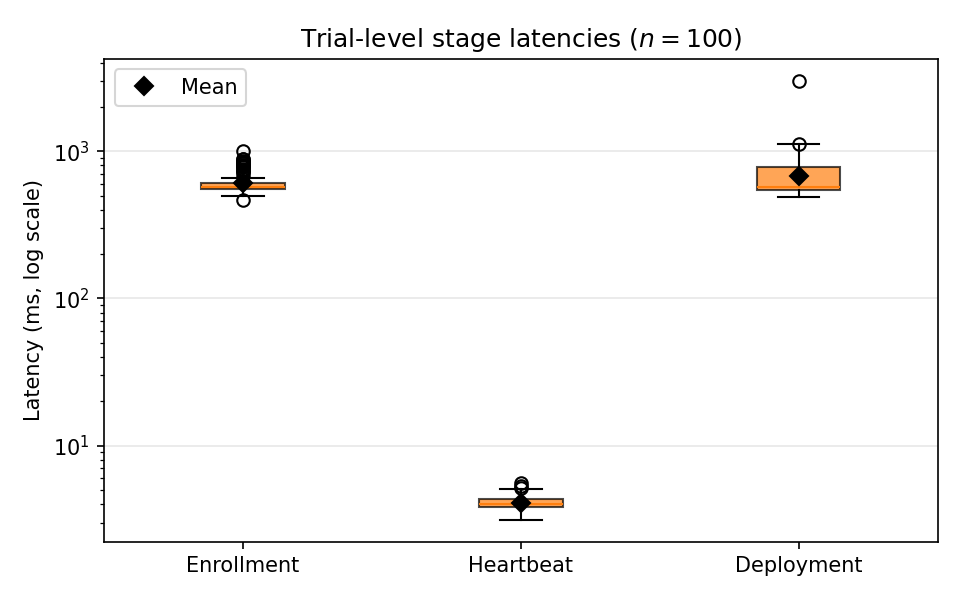
\includegraphics[width=\columnwidth]{figures/latency_boxplot.png}
\caption{Distribution of trial-level stage latencies ($n{=}100$, log scale). Diamonds indicate sample means.}%
\label{fig:latency-boxplot}
\end{figure}

\begin{figure}[pos=t]
\centering
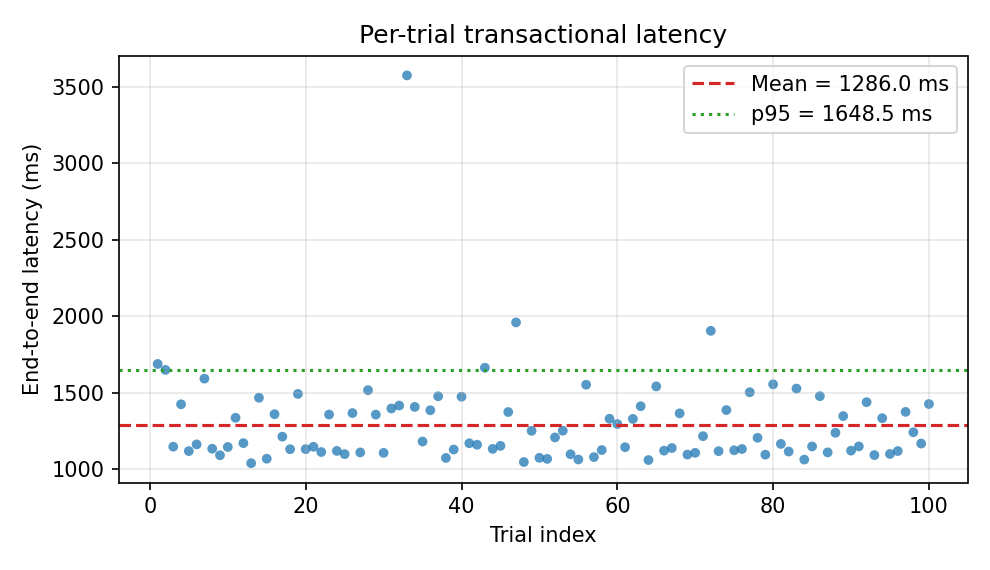
\includegraphics[width=\columnwidth]{figures/latency_trial_scatter.png}
\caption{\revC{End-to-end latency by trial index ($n{=}100$). The series is stationary after the discarded warm-up run; see Section~\ref{sec:evaluation} for the correlation statistics.}}%
\label{fig:latency-trial-scatter}
\end{figure}

\begin{figure}[pos=t]
\centering
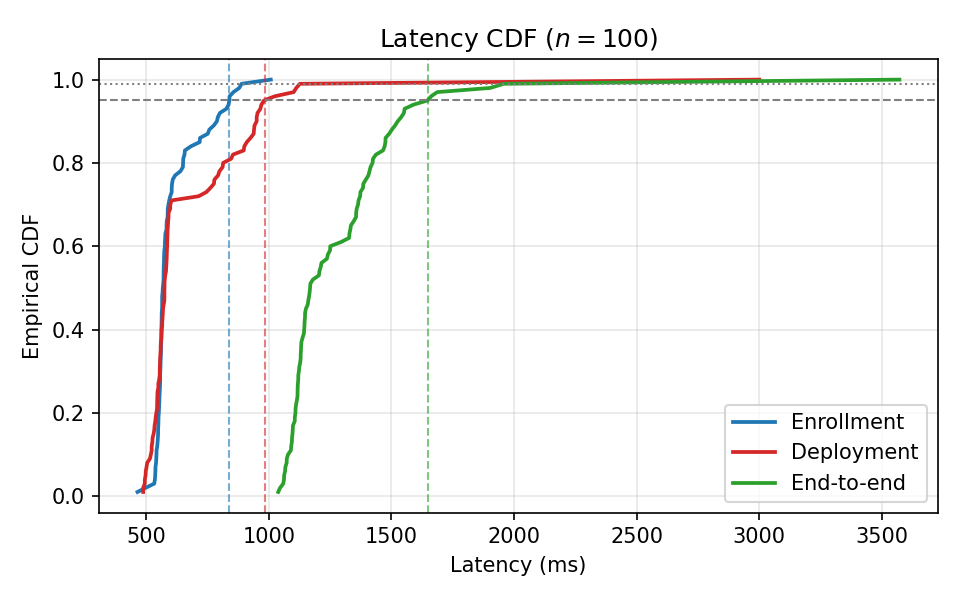
\includegraphics[width=\columnwidth]{figures/latency_cdf.png}
\caption{Empirical CDF of enrollment, deployment, and end-to-end latencies ($n{=}100$).}%
\label{fig:latency-cdf}
\end{figure}

\subsection{Sustainability-Oriented Metrics}\label{sec:sustainability-metrics}

\subsubsection{Southbound wire efficiency}
Application messages use a 4-byte big-endian length prefix followed by CBOR payloads. Figure~\ref{fig:wire-sizes} summarizes measured wire sizes for representative messages. Heartbeat request and acknowledgment are 6~B each; a complete enrollment round trip totals 87~B of application payload; a minimal deploy round trip (33~B WASM module) totals 90~B. % Removed: At the configured 25~s heartbeat period, steady-state control traffic is $12 \times (3600/25) = 1728$~B/h per device (${\approx}$1.69~KiB/h), excluding TLS record overhead.
{\color{red}At the configured 25~s heartbeat period, steady-state application-layer heartbeat traffic is $12 \times (3600/25) = 1728$~B/h per device (${\approx}$1.69~KiB/h), excluding TLS record overhead and lower-layer TCP/IP, Ethernet/TAP, and retransmission overhead.}

\revD{Because that exclusion spans more than an order of magnitude, we state the on-wire
cost analytically from the protocol constants, and mark it as an estimate rather than a
measurement. Under the evaluated TLS~1.2 AES-128-GCM cipher suite each record adds 5~B of
record header, an 8~B explicit nonce and a 16~B authentication tag, so a 6~B heartbeat
becomes a 35~B record, a 75~B IPv4 segment and a 93~B Ethernet frame. At a 25~s period the
delayed-acknowledgment timer expires between exchanges, so request and acknowledgment are
each acknowledged separately, giving roughly 300~B per heartbeat exchange and of order
40~KB/h per device: approximately $25\times$ the application-layer figure. Session
establishment is excluded from both numbers and is paid again on every reconnection, so a
device that re-handshakes frequently is dominated by that cost rather than by heartbeats.
A packet-capture measurement of steady-state and reconnection traffic, which would replace
this estimate, is left to future work.}

\begin{figure}[pos=t]
\centering
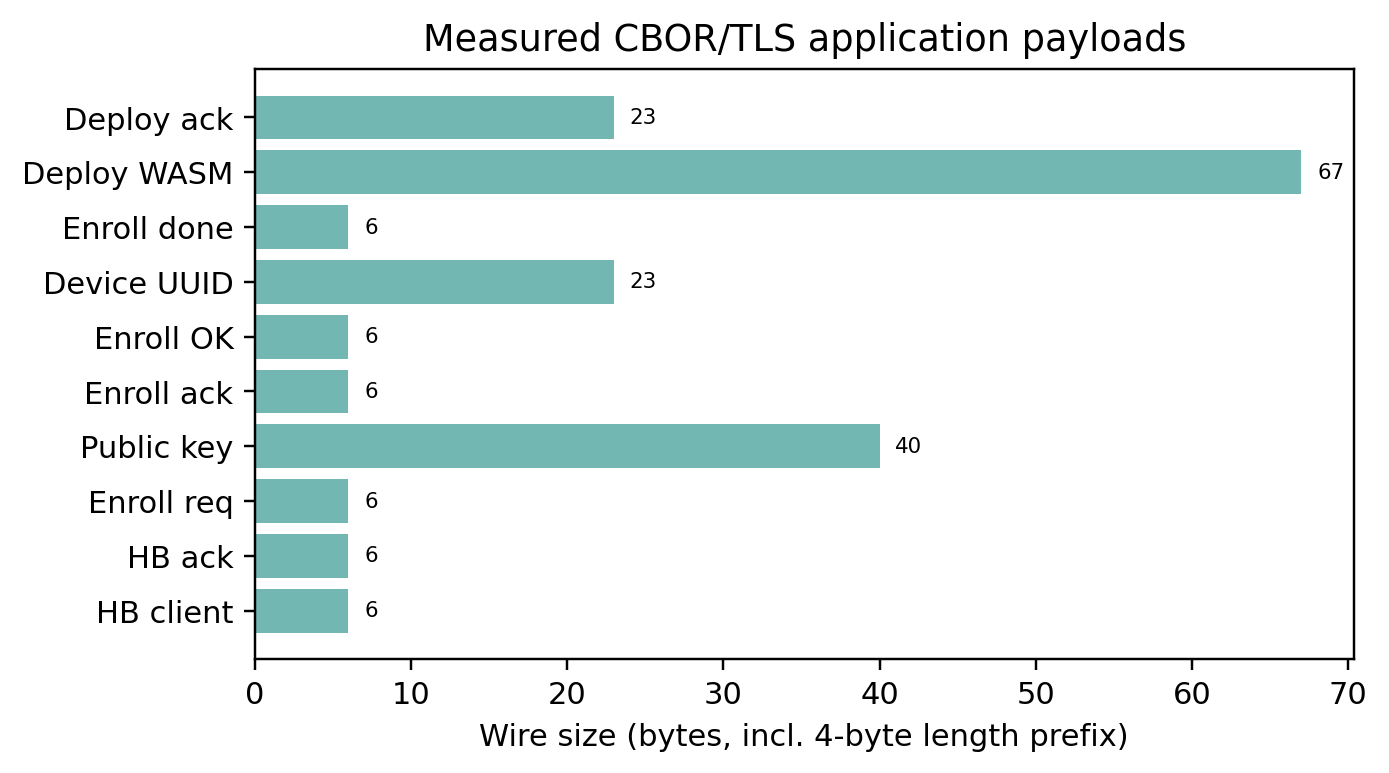
\includegraphics[width=\columnwidth]{figures/wire_sizes_bar.png}
\caption{Application-layer wire sizes (4-byte length prefix + CBOR) for representative protocol messages.}%
\label{fig:wire-sizes}
\end{figure}

\subsubsection{Edge footprint}
\begingroup
\color{red}
The evaluated Zephyr/WAMR/TLS/CBOR firmware fits the STM32F746NG internal-memory budget: the flash-resident \texttt{zephyr.bin} image is 406{,}568~B ($\approx$397~KiB), corresponding to text plus initialized data, and the static RAM allocation is 270{,}238~B ($\approx$264~KiB), corresponding to data (9{,}384~B) plus BSS (260{,}854~B).\footnote{The \texttt{zephyr.elf} file is 8{,}095{,}176~B (7.72~MiB), but only because it carries ELF metadata and debug symbols for the Renode \texttt{sysbus LoadELF} workflow; it is not the image written to device flash.} The benchmark WASM module remains 33~B. The architectural point supported by these measurements is therefore that embedded endpoints run no kubelet, container runtime, or Linux userspace while retaining an embedded-class memory footprint.
\endgroup


\subsubsection{Concurrent devices}\label{sec:concurrent-devices}
\begingroup
\color{red}
The trials above repeat one device through the full workflow, which measures the
workflow but says nothing about concurrency. A separate pass therefore attaches three
emulated STM32F746G devices at the same time. Each device carries its own enrollment
key, its own link-layer identity and its own DHCP lease, so the gateway, the control
plane and the network segment can all tell them apart; the identity a device presents
during enrollment is the one recorded in its Device resource.

All three attach and stay attached. The gateway runtime view lists three distinct
sessions, each with a heartbeat fresher than the 25~s firmware emission interval,
and the three Device resources independently reach \texttt{phase}\,=\,\texttt{Connected}
with their own liveness evidence. A single Application targeting all three devices
converges to \texttt{Running} on each of them: the gateway dispatches three separate
\texttt{DeployApplication} messages, one per session, and receives three successful
deployment acknowledgments. Because a deployment command travels only over the session
that belongs to its target device, three acknowledged deployments are direct evidence
of three independent southbound channels rather than of one channel reused.

Three devices on a single emulation host exercise session multiplexing, per-device
identity binding and per-device dispatch, establishing concurrency at the mechanism
level; Section~\ref{sec:discussion} states what this does not characterize.
\endgroup

\subsubsection{Control-plane resources}
Figure~\ref{fig:pod-resources} reports mean Kubernetes pod usage ($n{=}5$ samples, one TLS-connected device, sampled while the trial campaign was running). {\color{red}The metric is the container working set reported by \texttt{metrics-server}, cross-checked against cgroup~v2 \texttt{memory.current} and the anonymous resident set in \texttt{memory.stat}, which agree with it to within a few hundred kilobytes.} The gateway averaged 3.0~millicores CPU and 4.4~MiB RAM (\texttt{memory.current} 5.60~MB, anonymous 3.82~MB), the API server averaged 169.2~millicores and 33.4~MiB under campaign load (\texttt{memory.current} 32.3--33.0~MB), and the application controller averaged 38.4~millicores and 12.0~MiB (\texttt{memory.current} 13.3~MB). %Removed (minore): Registering 50 synthetic boards through the gateway HTTP registry left gateway resident memory unchanged (\texttt{memory.current} identical before and after), indicating lightweight per-device mediation state at the fog layer.
\revD{Registering 50 synthetic boards through the gateway HTTP registry left gateway
resident memory unchanged. This bounds the cost of registry state only: the boards are
\texttt{Device} entries rather than TLS-connected sessions, so the observation says nothing
about the per-session cost that would dominate a real fleet.}

\begin{figure}[pos=t]
\centering
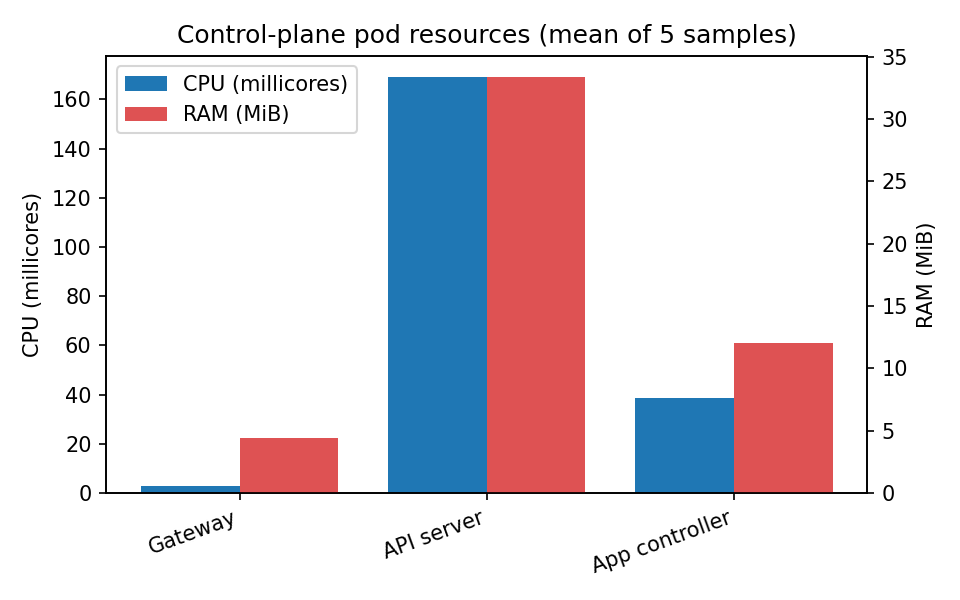
\includegraphics[width=\columnwidth]{figures/pod_resources_bar.png}
\caption{Mean CPU (millicores) and RAM (MiB) for control-plane pods during the sustainability measurement pass.}%
\label{fig:pod-resources}
\end{figure}

\begingroup
\color{blue}
\subsubsection{Computational energy instrumentation \revC{(measured CPU-time; derived energy and carbon as illustrative proxies)}}\label{sec:energy-instrumentation}
Beyond control-plane pod resources, we instrument a representative WASM computational workload directly. A Kubernetes pod running the fuel-metered Wasmtime runtime (\texttt{wasmbed-wasm-runtime}) repeatedly creates an isolated instance and executes a bounded arithmetic-loop WASM function (summing $0$ to $N$), cycling 30~s idle and 30~s active phases. This instruments a control-plane/fog-layer WASM execution path as a computational-energy proxy; 
%it does not measure the Renode-emulated STM32F746G/Zephyr/WAMR device evaluated elsewhere in this paper, since the embedded target is not directly instrumentable for energy in the present testbed. 
The pod runs under Guaranteed QoS (\texttt{requests}\,=\,\texttt{limits}, 2 vCPU) to remove self-induced CFS-throttling variance observed at the original 1-vCPU limit (835/27{,}021 accounting periods throttled under load, a scheduling artifact of the container's own quota, not of co-located tenants).

Two independent signals are collected. First, cgroup CPU time (\texttt{cpu.stat} \texttt{usage\_usec}) is an exact kernel accounting figure, not an estimate: at $N{=}200{,}000$, across $n{=}39$ paired cycles, the pod consumed $29.9289\pm0.0189$~CPU-s during each 30~s active window versus $0.000116\pm0.000053$~CPU-s during each equal-length idle window (paired difference 95\% CI $[29.9230, 29.9354]$~s, excluding zero). Second, we deploy Kepler~\cite{kepler} as a DaemonSet and query \texttt{kepler\_container\_joules\_total\{mode="dynamic"\}} scoped to the probe pod's own \texttt{pod\_name} label, isolating it from co-located wasmbed pods in the same namespace. 
Because the host is a virtualized guest without exposed RAPL counters, Kepler's output is a regression-based power estimate rather than a direct hardware measurement; with that caveat, it shows a clear and physically plausible increase under load: it attributes no dynamic power to the pod during the idle windows and $3.952$~W during the active ones (Figure~\ref{fig:energy-idle-active}). {\color{red}The exactly-zero idle attribution is a property of the estimator, not a measurement of the pod drawing no power.} We therefore treat the exact cgroup CPU-time as the primary, reproducible quantity throughout, and the Kepler wattage as a secondary, model-based signal consistent with it.

\begin{figure}[pos=t]
\centering
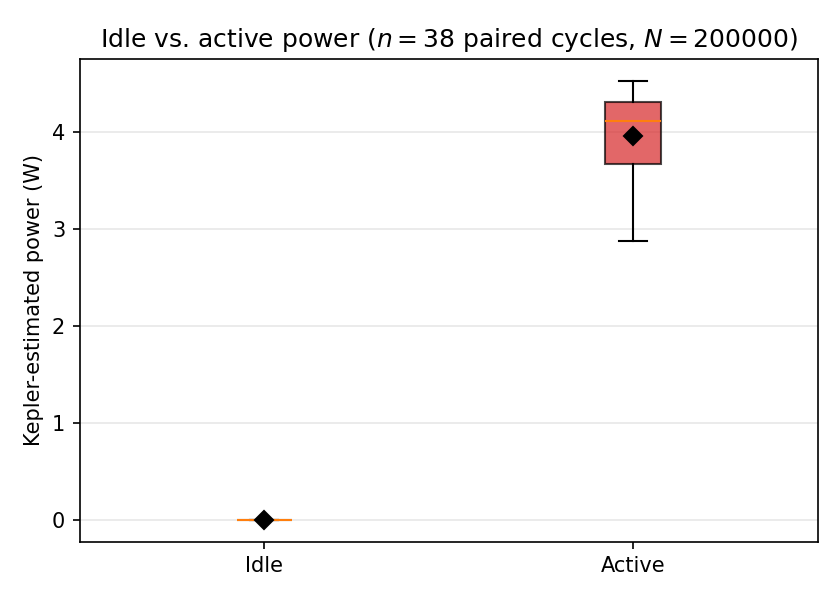
\includegraphics[width=\columnwidth]{figures/energy_idle_active_kepler.png}
\caption{Kepler-estimated power, idle vs.\ active phase ($n{=}38$ paired 30~s cycles with a power reading, $N{=}200{,}000$). Model-based estimate: this host exposes no RAPL counters.}%
\label{fig:energy-idle-active}
\end{figure}

Repeating the same idle/active protocol while varying the workload size $N \in \{50{,}000,\, 200{,}000,\, 1{,}000{,}000,\, 5{,}000{,}000\}$ ($n{\geq}10$ cycles per size) isolates CPU-time per WASM invocation from the fixed 30~s window: it grows from $95.9\,\mu$s at $N{=}50{,}000$ to $9.36$~ms at $N{=}5{,}000{,}000$. {\color{red}The two largest sizes exceed the MCU profile's default Wasmtime fuel budget of $5\times10^{6}$ units, which traps the call; they are measured with the budget raised (fuel metering still enabled), a change that alters no other aspect of the workload.} Plotted against an $O(N)$ reference line of slope~1 anchored at the smallest measured point, the four measurements track it closely across two orders of magnitude in $N$, consistent with the loop's linear time complexity rather than merely connecting four samples (Table~\ref{tab:workload-cpu-time}; 95\% CIs per point are narrower than the marker at this scale, $n{\geq}10$ cycles each).

\begin{table}[pos=t]
\centering
\caption{Workload size vs.\ measured CPU-time per invocation. \revC{CPU-s/call is exact kernel accounting; J/call is an \emph{illustrative range} spanning the two candidate per-vCPU full-load coefficients (4.72~W measured on the same part by a third party~\cite{epyc7313power}, 4.84~W from the manufacturer TDP~\cite{amd_epyc7313p}), and is read as an order of magnitude, not as a measurement.}}%
\label{tab:workload-cpu-time}
\footnotesize
\setlength{\tabcolsep}{3pt}
\begin{tabular}{rrrr}
\toprule
\textbf{$N$} & \textbf{$n$} & \textbf{CPU-s/call} & \revC{\textbf{J/call (illustrative)}} \\
\midrule
50{,}000 & 10 & $9.59\times10^{-5}$ & \revC{$4.5$--$4.6\times10^{-4}$} \\
200{,}000 & 39 & $3.77\times10^{-4}$ & \revC{$1.8\times10^{-3}$} \\
1{,}000{,}000 & 10 & $1.87\times10^{-3}$ & \revC{$8.8$--$9.0\times10^{-3}$} \\
5{,}000{,}000 & 10 & $9.36\times10^{-3}$ & \revC{$4.4$--$4.5\times10^{-2}$} \\
\bottomrule
\end{tabular}
\end{table}

Converting CPU-seconds into Joules requires a hardware-specific power coefficient, and this is the one step of the pipeline that is not measured on this platform. We therefore state its provenance explicitly. The primary reference is the manufacturer specification for the deployed processor, the AMD EPYC 7313P: 16 cores / 32 threads with a default TDP of 155~W and a configurable TDP of 155--180~W~\cite{amd_epyc7313p}, %Removed (minore): giving 4.84~W per vCPU at the default TDP.
giving 4.84~W per vCPU at the default TDP. \revD{The coefficient assumes that one vCPU
of the KVM guest of Table~\ref{tab:testbed} maps to one hardware thread of the host part,
which holds when the guest is not oversubscribed: the 32~vCPU guest matches the 32 threads
of the single socket. Under contention from other guests the effective per-vCPU power
would be lower than stated.} TDP is a thermal design limit rather than an instantaneous power draw, so it bounds rather than predicts consumption; as secondary corroboration, a third-party RAPL/\texttt{turbostat} measurement of the same single-socket part reports 35~W idle and 151~W full load across 32 threads~\cite{epyc7313power}, i.e.\ 1.09~W and 4.72~W per vCPU, within 3\% of the specification-derived value. Neither figure is a measurement of this workload on this hardware, and a platform-specific coefficient would come from a documented energy benchmark such as SPECpower\_ssj2008~\cite{specpower} or the per-family coefficient table of the Cloud Carbon Footprint project~\cite{ccf}. \revC{The conversion also rests on a deliberately simple model --- power proportional to allocated vCPU-time at full load --- which ignores the idle baseline, DVFS and turbo behaviour, shared uncore, memory and I/O power, and the known non-linearity of power against utilization. Each effect can move the result by tens of percent in either direction, which is why every derived figure below is given to at most two significant digits; removing the assumption requires re-anchoring the pipeline on a host exposing RAPL counters.}
Applying the Cloud Carbon Footprint average-wattage formula~\cite{ccf} to the measured utilization yields \revC{${\approx}119$}~J attributable to the active window above its idle baseline (\revC{${\approx}1.5$}~mJ per WASM invocation over ${\approx}$79{,}300 invocations per window). Carbon follows from that energy and a grid emission factor, and is reported here parametrically for the same reason: at an intensity $I$, the active window accounts for \revC{${\approx}33\,I$}~$\mu$gCO\textsubscript{2}eq with $I$ in gCO\textsubscript{2}eq/kWh. We take $I$ from the institutional source for Italy, the ISPRA national consumption-mix emission factor, 199.61~gCO\textsubscript{2}eq/kWh for 2025 (preliminary estimate)~\cite{ispra_settore_elettrico}, which puts the active window at \revC{${\approx}6.6$~mgCO\textsubscript{2}eq (of order $0.1$~$\mu$gCO\textsubscript{2}eq per invocation)}. Production- and consumption-mix factors differ and the choice must be stated with the value; the European Environment Agency indicator~\cite{eea_grid_intensity} provides the corresponding cross-country basis. 
%\revC{The measured claims of this subsection are therefore the CPU-time quantities alone; everything in Joules or grams of CO\textsubscript{2}eq is a proxy computed from them with an external coefficient, and no conclusion of this paper depends on its absolute value.}

\paragraph{Per-phase, per-pod CPU-time (control-plane trials).} %Removed (minore): As a minimal, additive instrumentation point layered on the trial harness behind Table~\ref{tab:quantitative-latency} (no change to gateway, controller, or reconciler logic), each
\revD{As an instrumentation point layered on the trial harness behind Table~\ref{tab:quantitative-latency}, leaving gateway, controller and reconciler logic unchanged, each} of the enrollment, heartbeat, and deployment stages is separately bracketed by a \texttt{cpu.stat} \texttt{usage\_usec} snapshot for the gateway, API-server, and application-controller pods, giving CPU-seconds consumed by each pod during exactly that stage's wall-clock window. %Removed (M8): The measurement runs against the full live stack: a Zephyr~3.5.0/WAMR firmware image for the emulated STM32F746G target, connected to the gateway over TLS through the Renode TAP bridge.
\revD{The measurement runs against the full live stack: a Zephyr~3.5.0/WAMR firmware
image for the emulated STM32F746G target, connected to the gateway over TLS through the
Renode TAP bridge. The two provisioning paths mentioned above are not alternatives here
but successive steps of the same trial. The board is first registered through the gateway's
auxiliary HTTP endpoint, which creates the \texttt{Device} resource and its expected
identity; the firmware then attaches over TLS and drives the same enrollment exchange as
the campaign of Table~\ref{tab:quantitative-latency}, so each record carries both a
registered board and a \texttt{Device} that reaches \texttt{phase}\,=\,\texttt{Connected}
with a fresh heartbeat. The difference from the main campaign is that registration is
performed explicitly rather than assumed from a pre-existing resource, which shifts a small
and constant amount of API-server work into the enrollment window; the stages themselves
are the same, and the two sets of latencies are not intended to be compared.} Table~\ref{tab:cpu-time-per-phase} reports a $n{=}5$-trial pass: all three stages succeed 5/5, with real, reproducible CPU-time per stage per pod, and the enrollment row covers the full protocol exchange (TLS handshake, CBOR EnrollmentRequest/PublicKey/DeviceUuid, gateway-side connection established) up to the Device CRD reaching \texttt{status.phase}\,=\,\texttt{Connected}.

Given $n{=}5$, this table demonstrates the instrumentation working end-to-end on real infrastructure rather than providing a statistically powered per-stage estimate; a $n{=}100$ run aligned with Table~\ref{tab:quantitative-latency} is future work.

\begin{table}[pos=t]
\centering
%Removed (M8): \caption{CPU-seconds per phase per pod ($n{=}5$ trials, \revC{provisioned through the auxiliary HTTP registry endpoint}; all three stages succeeded 5/5). Exact cgroup \texttt{cpu.stat}, not an estimate.}%
\caption{CPU-seconds per phase per pod ($n{=}5$ trials, \revD{board registered through the gateway HTTP endpoint and then enrolled over TLS}; all three stages succeeded 5/5). Exact cgroup \texttt{cpu.stat}, not an estimate.}%
\label{tab:cpu-time-per-phase}
\footnotesize
\setlength{\tabcolsep}{2pt}
\resizebox{\columnwidth}{!}{%
\begin{tabular}{llrrrr}
\toprule
%Removed (M8): colonne p95 e IC-t sostituite da min--max e bootstrap; valori originali:
%\textbf{Stage} & \textbf{Pod} & \textbf{Mean} & \textbf{Median} & \textbf{p95} & \textbf{95\% CI of mean} \\
%Enrollment & gateway & 0.000350 & 0.000326 & 0.000503 & [0.000239, 0.000462] \\
%Enrollment & api-server & 0.143510 & 0.083265 & 0.384413 & [$-$0.023697, 0.310717] \\
%Enrollment & app-controller & 0.036625 & 0.035557 & 0.045817 & [0.029140, 0.044109] \\
%Heartbeat & gateway & 0.000413 & 0.000390 & 0.000684 & [0.000206, 0.000620] \\
%Heartbeat & api-server & 0.020483 & 0.000000 & 0.102417 & [$-$0.036379, 0.077345] \\
%Heartbeat & app-controller & 0.010088 & 0.010080 & 0.010956 & [0.009043, 0.011133] \\
%Deployment & gateway & 0.006338 & 0.006521 & 0.008674 & [0.003693, 0.008984] \\
%Deployment & api-server & 0.564172 & 0.465255 & 0.823915 & [0.280249, 0.848096] \\
%Deployment & app-controller & 0.057557 & 0.027365 & 0.111654 & [$-$0.002620, 0.117734] \\
\textbf{Stage} & \textbf{Pod} & \textbf{Mean} & \textbf{Median} & \revD{\textbf{Min--max}} & \revD{\textbf{95\% CI (bootstrap)}} \\
\midrule
Enrollment & gateway & 0.000350 & 0.000326 & \revD{0.000266--0.000503} & \revD{[0.000291, 0.000432]} \\
Enrollment & api-server & 0.143510 & 0.083265 & \revD{0.080665--0.384413} & \revD{[0.082006, 0.264079]} \\
Enrollment & app-controller & 0.036625 & 0.035557 & \revD{0.030778--0.045817} & \revD{[0.032261, 0.041684]} \\
Heartbeat & gateway & 0.000413 & 0.000390 & \revD{0.000227--0.000684} & \revD{[0.000292, 0.000563]} \\
Heartbeat & api-server & 0.020483 & 0.000000 & \revD{0.000000--0.102417} & \revD{[0.000000, 0.061450]} \\
Heartbeat & app-controller & 0.010088 & 0.010080 & \revD{0.009197--0.010956} & \revD{[0.009415, 0.010760]} \\
Deployment & gateway & 0.006338 & 0.006521 & \revD{0.003787--0.008674} & \revD{[0.004659, 0.008018]} \\
Deployment & api-server & 0.564172 & 0.465255 & \revD{0.307216--0.823915} & \revD{[0.390794, 0.739244]} \\
Deployment & app-controller & 0.057557 & 0.027365 & \revD{0.019152--0.111654} & \revD{[0.021213, 0.093901]} \\
\bottomrule
\end{tabular}%
}
\end{table}
\endgroup

\subsubsection{Architectural comparison}
Table~\ref{tab:arch-compare} contrasts gateway-mediated WASM orchestration with treating each constrained device as a Kubernetes worker. % Removed: Edge Kubernetes deployments commonly require tens to hundreds of MiB of resident memory per worker for kubelet and container runtime before user workloads~\cite{kubernetes}.
{\color{red}Edge Kubernetes deployments require a Linux-capable node with a kubelet, container runtime, and supporting operating-system services before user workloads, whereas the evaluated endpoint keeps those cluster agents off the device.} %Removed (M6): Our design concentrates orchestration in a shared gateway (under 5~MiB measured) while keeping cluster agents off the device.
\revD{Our design concentrates orchestration in a shared gateway (under 5~MiB measured)
while keeping cluster agents off the device. The comparison is a qualitative contrast of
architectural models, not a measured benchmark: only the right-hand column is instrumented
here, and establishing the left-hand one would require running the same WASM workload on a
Linux single-board node with a cluster agent. The pod measurements also locate the real
cost differently from the intuition the table invites. Mediation is cheap---the gateway
averages 3.0~millicores---while the API server averages 169.2~millicores, so the
control plane, not the fog layer, dominates control-plane CPU at this scale. Whether
gateway mediation remains cheaper than per-device agents therefore depends on fleet size
through a break-even this evaluation does not determine.}

\begin{table}[pos=t]
\centering
%Removed (M6): \caption{Orchestration model comparison.}%
\caption{\revD{Qualitative contrast of orchestration models. Only the gateway-mediated column is measured in this work.}}%
\label{tab:arch-compare}
\footnotesize
\setlength{\tabcolsep}{3pt}
\begin{tabular}{p{0.22\linewidth} p{0.34\linewidth} p{0.34\linewidth}}
\toprule
\textbf{Aspect} & \textbf{Device as K8s worker} & \textbf{Gateway-mediated WASM edge} \\
\midrule
Edge runtime & kubelet + container runtime + OS & Zephyr + WAMR ({\color{red}397~KiB flash, 264~KiB RAM}) \\
% Removed: Edge cluster agent RAM & 100--350~MiB per node (literature) & none on device \\
{\color{red}Edge cluster agent footprint} & {\color{red}kubelet + container runtime + OS services required} & none on device \\
% Removed: Steady control traffic & CRI/container probes & 1728~B/h per device \\
{\color{red}Steady heartbeat traffic} & CRI/container probes & {\color{red}1728~B/h per device (application layer)} \\
Fog mediation RAM & per-node agent & ${<}5$~MiB shared gateway \\
\bottomrule
\end{tabular}
\end{table}

\section{Discussion}\label{sec:discussion}

\subsection{Architectural and RI Implications}
The main architectural lesson is that the gateway should be treated as a semantic boundary, not as a transparent relay. Constrained devices can remain focused on protected communication, local execution, and evidence emission, while the gateway handles identity validation, protocol translation, and status propagation toward Kubernetes. This separation avoids pushing cloud-facing semantics into firmware and gives the control plane a stable interface even if the southbound protocol evolves.

The evaluation confirms that protocol success alone is not sufficient: enrollment, liveness, and deployment evidence must be interpreted consistently before they become trustworthy control-plane state. This supports the central design decision to separate desired state, gateway-derived evidence, and controller reconciliation. Future extensions such as multi-gateway placement, staged rollout, or retry policies should preserve this separation rather than allowing multiple components to write conflicting interpretations of device status.

For sustainable digital research infrastructures, the same separation creates explicit attachment points for energy and carbon policies. Placement decisions can be expressed as desired state, gateway and device observations can be treated as evidence, and sustainability controllers can consume the same status model without requiring constrained devices to run additional cloud-native agents. The measured baselines in Section~\ref{sec:sustainability-metrics}, byte-scale southbound traffic, single-digit-MiB gateway mediation, and no kubelet on the edge, suggest that subsequent green-experimentation studies can focus on policy and instrumentation rather than on redesigning the orchestration substrate.

%{\color{red}For the scope of sustainable digital research infrastructures, the main outcome is therefore methodological rather than directly energetic: the paper identifies where orchestration evidence, device liveness, gateway mediation, and resource overhead can be captured consistently before energy-aware or carbon-aware decisions are automated.}

\begingroup
\color{red}
The practical implication for research infrastructures is that orchestration evidence becomes a reusable experimental object. A placement policy, for example, can be evaluated by inspecting which Application resources were scheduled to which devices, which gateway mediated the execution, whether heartbeat evidence remained fresh, and whether the reported execution outcome matched the intended state. The same record can later be joined with external measurements such as site power, carbon-intensity annotations, thermal constraints, or gateway utilization. The current prototype does not optimize those signals, but it provides the control-plane hooks that a sustainability-aware controller would need in order to make such optimization auditable.

%Removed (ridondanza): The gateway boundary also simplifies reproducibility. A reproduced experiment does not need the embedded device to expose Kubernetes-native behavior; it only needs the same southbound protocol semantics, the same CRD intent, and the same interpretation of evidence. This is useful for multi-site RIs, where physical boards, local networks, and energy meters may differ across laboratories. The orchestration claim can be retested with emulation, while hardware-specific claims can be added as separate measurement layers.

\endgroup

\subsection{Validity and Scope}
The validation targets system-level orchestration behavior rather than real-time performance, radio behavior, or sustainability optimization. Emulation and scripted trials are appropriate for exercising enrollment, deployment, status convergence, and reconciliation semantics, while physical boards, wireless links, and power meters require additional characterization. The results should therefore be interpreted as evidence that the orchestration model is coherent under the evaluated workflow.

% Removed: External validity is bounded by the single-node K3s deployment, one gateway path, and a representative minimal workload.
{\color{red}External validity is bounded by the single-node K3s deployment, one gateway path, and a minimal WASM workload selected to isolate orchestration overhead rather than application-computation cost.} Larger deployments introduce gateway contention, distributed failure modes, network partitions, and device mobility. % Removed: A supplementary scaling attempt with three Renode machines on the shared TAP test bed kept only one TLS session active in the gateway runtime view; fleet-scale energy characterization therefore requires isolated network segments or physical boards.
%Removed (compressione): {\color{red}Concurrency is exercised directly rather than assumed: three emulated devices attached simultaneously hold three distinct TLS sessions in the gateway runtime view and each receive their own deployment (Section~\ref{sec:concurrent-devices}). The 50-board registry exercise remains a registry-state scaling check, since those boards are registry entries rather than TLS-connected devices, and the concurrency evidence stops at the three devices actually measured on a single host: it does not license extrapolation to hundreds of devices, to multiple gateways, or to fleet-scale energy characterization, all of which remain open.}
{\color{red}Concurrency is exercised rather than assumed: three emulated devices hold
three distinct TLS sessions and each receives its own deployment
(Section~\ref{sec:concurrent-devices}). That evidence stops at three devices on one host,
and the 50-board exercise scales registry state rather than sessions, so neither extends to
multiple gateways or to fleet-scale energy characterization.} Construct validity is also scoped: the study measures %Removed (M11): "secure attachment"
\revD{identity-bound attachment}, observable liveness, deployment completion, latency, wire sizes, firmware footprint, and control-plane RAM/CPU samples, while direct, hardware-validated energy consumption and long-duration reliability remain outside the current evaluation%Removed (compressione): {\color{blue}; Section~\ref{sec:energy-instrumentation} reports a computational-energy instrumentation pass on a representative WASM workload using exact cgroup CPU-time as the primary signal and a model-based Kepler host-power estimate as a secondary one, as a step toward that validation.}
{\color{blue}; Section~\ref{sec:energy-instrumentation} is a step toward the latter, with exact cgroup CPU-time as the primary signal.}

\begingroup
\color{blue}
\paragraph{Scope of the energy signal.} cgroup CPU-time (\texttt{cpu.stat}) is the only quantity in Section~\ref{sec:energy-instrumentation} that is an exact, reproducible measurement rather than a model output, and it alone should be treated as load-bearing for any energy claim in this paper. 
%The Kepler wattage is a secondary, corroborating signal: this VM exposes no RAPL counters, so every reported watt is the output of Kepler's regression-based power model rather than a hardware reading, independent of how large the sample is. The Joule and carbon figures in Table~\ref{tab:workload-cpu-time} are a further derived layer on top of the measured CPU-time, using a literature power coefficient, and are reported as illustrative estimates rather than measurements. 
A hardware-validated absolute wattage for this workload, on a host that combines a working k3s control plane with exposed RAPL counters, remains future work.
\endgroup

Conclusion validity is strengthened by the transactional success criterion: enrollment, heartbeat visibility, and deployment must succeed within the same trial. This avoids overstating correctness from isolated protocol stages. Broader claims about optimality, scalability, or comparative advantage require additional experiments against alternative orchestration designs and physical-device deployments.

\begingroup
\color{red}
\subsection{Scalability and Failure Modes}
The main scalability pressure point is the gateway, because it concentrates southbound sessions, protocol parsing, and status propagation. This is an intentional trade-off: moving the boundary into the gateway avoids embedding Kubernetes behavior in every device, but it also means that future deployments must treat gateways as schedulable and observable resources. Multi-gateway operation should therefore add explicit placement policies, per-gateway capacity metadata, and failover rules rather than relying on implicit network reachability. In such a design, a Device resource would declare or discover a preferred gateway, while Application reconciliation would resolve the current gateway association before attempting deployment.

%Removed (compressione): The evaluated system also identifies four categories of faults. Transport faults include TLS interruption, device reboot, and heartbeat loss. Protocol faults include malformed CBOR records, identity mismatch, stale session state, and deployment results that cannot be associated with the requested Application. Control-plane faults include delayed status patches, controller restarts, and conflicting updates from independent reconcilers. Application faults include WASM load failure, runtime error, or an execution result that does not satisfy the expected policy. Treating these cases separately is important because each one requires a different recovery action: reconnect, reject enrollment, retry deployment, preserve desired state, or surface an explicit error to the operator.
\revD{Four fault categories require distinct recovery actions and are therefore kept
separate: transport faults (TLS interruption, reboot, heartbeat loss) call for reconnection;
protocol faults (malformed CBOR, identity mismatch, stale sessions, unassociable deployment
results) for rejection; control-plane faults (delayed patches, controller restarts,
conflicting reconcilers) for preserving desired state; and application faults (WASM load
failure, runtime error, policy violation) for surfacing an explicit error.}

%Removed (artefatto): The above-stated considerations also limits the interpretation of the present results.
\revD{These considerations also limit the interpretation of the present results.} The 100-trial campaign shows that the nominal enrollment-to-deployment transaction is coherent under the evaluated emulated conditions. It does not establish maximum gateway capacity, behavior under network partitions, real-time scheduling guarantees, or recovery time after simultaneous failures. Those are natural next experiments once the single-device protocol and reconciliation invariants are fixed.
\endgroup

\subsection{Reproducibility}
The evaluation is designed to be repeatable on a commodity Linux host with Docker and K3s. Renode makes the embedded side deterministic enough for regression-style validation, although it remains complementary to future physical-board experiments. Evidence traceability is maintained across multiple layers: gateway logs, API-visible resource states, and Kubernetes CRD status describe the same workflow from different perspectives, so that protocol success and control-plane convergence are not inferred from a single eventually consistent field.

\begingroup
\color{red}
For a replication package, the most important artifacts are therefore not only the source code and container images, but also the CRD manifests, firmware configuration, WASM module, trial harness, raw latency records, and the scripts that generate the figures. Reporting these artifacts together would allow another researcher to distinguish implementation regressions from environmental variation. A failed replication could then be localized to a specific layer: Kubernetes resource creation, gateway mediation, TLS/CBOR communication, embedded execution, or post-processing of the measurement records. {\color{red}If institutional constraints prevent publishing all raw records, the artifact statement should separate public assets, such as source code, manifests, and scripts, from records available on request.}
\endgroup

\section{Conclusion and Future Work}\label{sec:conclusion}

This paper presented a Kubernetes-native framework for managing embedded WebAssembly workloads across the Cloud\textendash{}Fog\textendash{}Edge continuum without requiring constrained devices to become Kubernetes nodes. The contribution integrates CRD-based intent, gateway-mediated TLS/CBOR communication, Zephyr firmware, WAMR execution, and evidence-driven reconciliation into a single verifiable operational path suitable for sustainable digital research infrastructures.

% Removed: The experimental evaluation on a K3s test bed with emulated embedded targets confirms that the architecture supports a complete enrollment-to-deployment workflow under repeatable conditions, with 100/100 transactional success and {\color{red}approximately 1.29~s mean end-to-end orchestration latency}. Measured southbound control traffic, firmware footprint, and fog-layer resource use provide quantitative anchors for subsequent energy-aware placement and green-experimentation studies.
{\color{red}The experimental evaluation on a K3s testbed with emulated embedded targets confirms that the architecture supports a complete enrollment-to-deployment workflow under repeatable conditions, with 100/100 transactional success and approximately 1.29~s mean end-to-end orchestration latency. The measured application-layer traffic, firmware footprint, and fog-layer resource use provide quantitative anchors for subsequent energy-aware placement, carbon-aware annotation, and green-experimentation studies, while direct energy optimization remains future work.}
\revD{The computational-energy pass of Section~\ref{sec:energy-instrumentation} should be
read with the same scope: it instruments a Wasmtime runtime at the fog layer, not the
Zephyr/WAMR firmware on the embedded target, and its Joule and carbon figures are proxies
derived from measured CPU-time with an external power coefficient. No energy measurement
on the constrained endpoint itself is claimed.}

Future work will extend the platform toward multi-gateway deployments, fault injection, physical hardware, wattmeter- or RAPL-validated energy measurements{\color{blue}, carbon-intensity annotation beyond the illustrative, derived-estimate pass reported in Section~\ref{sec:energy-instrumentation}}, and larger device populations.

\section*{Data Availability Statement}
The data supporting the findings of this study consist of deployment logs, Kubernetes resource states, controller and gateway traces, and protocol evidence from controlled experiments. % Removed: Anonymized records, validation workflows, and accompanying documentation are available from the corresponding author upon reasonable request, subject to institutional policies and applicable confidentiality constraints.
\revC{The source repository provides the public deployment assets needed to inspect the framework. The measurement artifacts underlying every number reported in Section~\ref{sec:evaluation} --- the per-trial latency and success records of the $n{=}100$ campaign, the paired idle/active and workload-size energy records, the per-phase \texttt{cpu.stat} records, the pod-resource samples, and the analysis and figure-generation scripts that turn them into the tables and figures of this paper --- are deposited as a single versioned archive on Zenodo under DOI \texttt{10.5281/zenodo.XXXXXXX} (release \texttt{v1.0}, CC~BY~4.0), and the corresponding source tree is archived in Software Heritage under identifier \texttt{swh:1:rev:XXXXXXXX}. The deposit is immutable and citable; the GitHub repository below is its development mirror and may advance beyond the archived release. Records not included in the deposit are limited to raw operational logs that carry institutional infrastructure identifiers; these are available from the corresponding author upon reasonable request, subject to institutional policies and applicable confidentiality constraints.}

\section*{Code Availability Statement}
The source code and deployment assets associated with the framework are maintained in the public project repository \href{https://github.com/lucadagati/k3s-wasm-edge-orchestration}{\nolinkurl{lucadagati/k3s-wasm-edge-orchestration}}. \revC{The exact revision evaluated in this paper is tagged \texttt{v1.0} and archived, together with the measurement artifacts and analysis scripts, under the Zenodo DOI and Software Heritage identifier given in the Data Availability Statement, so that the results can be reproduced from a fixed, citable snapshot rather than from a moving branch.}

% TODO before submission: mint the Zenodo DOI and the Software Heritage identifier for tag v1.0
% and replace the XXXXXXX placeholders above and in the Data Availability Statement.

\section*{Funding}
This research received no external funding.

\section*{Conflict of Interest}
The authors declare that they have no conflict of interest related to this work.

\section*{Author Contributions}
Conceptualization: Giovanni Merlino, with input from Francesco Longo. Methodology: Luca D'Agati, Giuseppe Tricomi, Fabio Orazio Mirto, and Giovanni Merlino. Software: Luca D'Agati, with contributions from Giuseppe Tricomi and Fabio Orazio Mirto. Validation: Luca D'Agati, Giuseppe Tricomi, and Fabio Orazio Mirto. Investigation and data curation: Luca D'Agati, Giuseppe Tricomi, and Fabio Orazio Mirto. Writing---original draft: Luca D'Agati, with writing support from Giuseppe Tricomi and Fabio Orazio Mirto. Writing---review and editing: Luca D'Agati, Giuseppe Tricomi and Fabio Orazio Mirto. Supervision: Giovanni Merlino, with support from Francesco Longo.


\bibliographystyle{els-cas-templates/cas-model2-names}
\bibliography{references}

\end{document}
